\documentclass[a4paper,12pt]{report}
\renewcommand\thesection{\arabic{section}}
\renewcommand{\contentsname}{Cuprins}
\renewcommand{\figurename}{Figura}
\renewcommand{\tablename}{Tabel}
\usepackage{amsmath}
\usepackage{rotating}
\usepackage{listings}
\usepackage{lipsum}  
\usepackage{titlesec}
\titleformat{\section}[hang]{\normalfont\Large\bfseries}{\thesection}{1em}{}
\titleformat{\subsection}[hang]{\normalfont\large\bfseries}{\thesubsection}{1em}{}
\titleformat{\subsubsection}[hang]{\normalfont\normalsize\bfseries}{\thesubsubsection}{1em}{}


\setcounter{tocdepth}{6}
\setcounter{secnumdepth}{6}

\usepackage{url}
\usepackage[backend=bibtex,style=numeric,citestyle=numeric,backref=true,sorting=none]{biblatex}
\addbibresource{bibliography.bib}

\usepackage{indentfirst}
\usepackage[nobottomtitles*]{titlesec}

\newcommand*{\justifyheading}{\raggedleft}
\titleformat{\section}{\normalfont\Large\justifyheading}{\thesection}{18pt}{}

\usepackage{graphicx}
\usepackage[export]{adjustbox}
\graphicspath{ {./images/} }

\usepackage[center]{caption}
\usepackage{subcaption}
\usepackage{hyperref}

\usepackage[margin=3.9cm]{geometry}

\usepackage{listings}
\usepackage{color}
\usepackage{float}

\definecolor{codegreen}{rgb}{0,0.6,0}
\definecolor{codegray}{rgb}{0.5,0.5,0.5}
\definecolor{codepurple}{rgb}{0.58,0,0.82}
\definecolor{backcolour}{rgb}{0.96,0.96,0.96}

\lstdefinestyle{mystyle}{
	backgroundcolor=\color{backcolour},   
	commentstyle=\color{codegreen},
	keywordstyle=\color{blue},
	numberstyle=\tiny\color{codegray},
	stringstyle=\color{codepurple},
	basicstyle=\fontsize{10}{10}\selectfont\ttfamily,
	breakatwhitespace=false,         
	breaklines=true,                 
	captionpos=b,                    
	keepspaces=true,                 
	numbers=left,                    
	numbersep=2pt,                  
	showspaces=false,                
	showstringspaces=false,
	showtabs=false,                  
	tabsize=2
}

\lstset{style=mystyle}

\usepackage{pythonhighlight}

\usepackage{fontspec} % -> Schimbat compilator in LuaLatex
\setmainfont{[UTSans-Regular.otf]}
\usepackage{setspace}
\usepackage{tocloft}
\setstretch{1}

% Personalizare cuprins
\renewcommand{\cftchapfont}{\bfseries\normalsize} % Font pentru capitole
\renewcommand{\cftsecfont}{\normalsize} % Font pentru secțiuni
\renewcommand{\cftsubsecfont}{\small} % Font pentru subsecțiuni
\renewcommand{\cftdotsep}{1.5} % Distanța între titlu și pagină (puncte)

\renewcommand{\cftchappagefont}{\bfseries\normalsize} % Font număr de pagină capitole
\renewcommand{\cftsecpagefont}{\normalsize} % Font număr de pagină secțiuni
\renewcommand{\cftsubsecpagefont}{\small} % Font număr de pagină subsecțiuni

\begin{document}

\begin{titlepage}
	
	\vspace*{-3cm}
	\hspace{-2cm}
	
\includegraphics[width=0.8\linewidth]{./images/Logo-UT-IESC-SPOT-RO}
		
		\vspace{2cm}
		\begin{center}
		\Huge\textbf{Sistem de acces cu recunoaștere
facială folosind Arduino}
        \end{center}
		
		\vfill
				
        \noindent\Large{Conducător științific: CIOBANU CĂTALIN BOGDAN}\hfill \\ 
        \Large{Titulatura. SEF LUCRARI UNIVERSITAR}\hfill \\
        \begin{center}
        \hfill\Large{Studenți:} \\
        \hfill\Large{Ionescu Rareș-Ionuț} \\
        \hfill\Large{Brujbeanu Gabriel-Lucian} \\
        
       
        \end{center}
		
		\vfill
		
		\Large
        \begin{center}
		\textbf{Brașov, 2025}
        \end{center}
        
\end{titlepage}
\include{./cover/innercover}

\newpage
\setcounter{page}{2}

% Cuprins automat cu personalizare și puncte
\tableofcontents
\newpage

% Continuare document
\pagenumbering{arabic}

\chapter*{Rezumat}
\addcontentsline{toc}{chapter}{Rezumat}

Scopul acestui proiect este de a implementa un sistem de acces controlat prin recunoașterea facială, utilizând o placă Arduino Uno și perifericele sale. Proiectul își propune să demonstreze utilizarea registrelor și a programării la nivel hardware pentru controlul unor periferice cum ar fi un motor servo și să ofere o soluție practică pentru securitatea fizică. 

De asemenea, se urmărește învățarea și aplicarea conceptelor de recunoaștere facială și control automatizat al accesului, precum și utilizarea componentelor de feedback vizual, cum ar fi LCD-ul și LED-urile, cât și reglarea intensității acestora cu ajutorul unui potențiometru. În același timp, proiectul oferă oportunitatea de a lucra cu limbajul de programare Python, deoarece conține un mic script folosit pentru recunoașterea facială, care preia imaginile captate de ESP, de la URL-ul generat prin Espressif, iar apoi, în funcție de verificare, transmite mesajele corespunzătoare dispozitivelor de ieșire.

Astfel, proiectul oferă studenților mai multe posibilități de dezvoltare și aprofundare. Pe de o parte, este vorba despre partea hardware, în care studenții vor învăța modul în care interacționează componentele între ele și legăturile dintre acestea datorită Arduino, iar pe de altă parte intervine partea de software prin programarea în limbajul Python. De asemenea, apare și programarea la nivel de regiștri, proiectul reprezentând astfel o posibilitate prin care studenții să își dea seama despre ramura care îi atrage mai mult, experimentând aici câte puțin din toate.

\newpage

\chapter*{INTRODUCERE}
\addcontentsline{toc}{chapter}{INTRODUCERE} % Adăugăm capitolul în cuprins

\section{Descrierea temei}
În cadrul acestui proiect, am dezvoltat un sistem de acces controlat prin recunoașterea facială, utilizând o platformă Arduino Uno și perifericele sale. Sistemul identifică persoanele prin procesarea imaginilor faciale, permițând accesul doar celor autorizați și asigurând un nivel ridicat de securitate fizică.

Proiectul implică utilizarea registrelor și a programării la nivel hardware pentru controlul unor componente cheie, precum motorul servo, care deschide o ușă, și sistemele de feedback vizual, incluzând LED-urile și ecranul LCD. Aceste componente sunt reglate și controlate printr-un potențiometru, ce permite ajustarea intensității semnalelor vizuale.

De asemenea, am integrat un modul de recunoaștere facială, care utilizează un script Python pentru preluarea și procesarea imaginilor captate de camera ESP32-CAM. Imaginile sunt comparate cu un set pre-stocat de imagini, iar în funcție de rezultatul verificării, se activează sau dezactivează diferite dispozitive de ieșire, precum motorul servo.

Prin dezvoltarea acestui sistem, am învățat și aplicat concepte importante din domeniul electronicii și programării. Am experimentat interacțiunea dintre componentele hardware, controlul perifericelor și programarea la nivel de registre. Proiectul reprezintă o oportunitate excelentă de aprofundare a cunoștințelor în domeniul tehnologiilor de recunoaștere facială și al controlului automatizat al accesului.

\section{Motivația practică pentru alegerea temei}
Alegerea temei pentru acest proiect a fost determinată de necesitatea implementării unor soluții moderne de securitate, care să răspundă cerințelor din ce în ce mai complexe ale protecției fizice în diverse medii. Recunoașterea facială reprezintă una dintre tehnologiile cele mai avansate și fiabile în domeniul autentificării, iar utilizarea acesteia într-un sistem de acces controlat este o aplicație practică relevantă pentru viitorul tehnologiilor de securitate.

În plus, tema a fost aleasă pentru a oferi o oportunitate de învățare și aplicare a unor concepte fundamentale în domeniul electronicii și programării, în special a programării la nivel hardware și a utilizării microcontrolerelor. Utilizarea platformei Arduino Uno, un instrument accesibil și extrem de versatil, permite integrarea rapidă și eficientă a componentelor hardware, cum ar fi motoarele servo, modulele LCD și LED-urile, toate controlate prin registre și programare la nivel de hardware.

De asemenea, integrarea unui sistem de recunoaștere facială prin intermediul unui script Python și a modulului ESP32-CAM adaugă un nivel de complexitate care permite aprofundarea cunoștințelor de programare, inclusiv în domeniul procesării imaginilor și al aplicațiilor de tip IoT (Internet of Things). Astfel, acest proiect oferă o oportunitate completă de învățare, acoperind atât partea de hardware, cât și de software, iar implementarea unui sistem de securitate bazat pe recunoaștere facială reprezintă un exemplu concret de aplicare a tehnologiilor emergente în viața reală.

\section{Sisteme Actuale}

În această secțiune, prezentăm două sisteme care au similarități cu proiectul propus, bazat pe recunoaștere facială și acționarea unui motor.

\subsection{Sistemul de control al accesului bazat pe recunoaștere facială}
\textbf{Descriere:} \\
Acest sistem este utilizat în organizații sau clădiri rezidențiale pentru a înlocui cheile fizice sau cardurile de acces. Un astfel de sistem folosește o cameră pentru a captura imaginea utilizatorului, algoritmi de recunoaștere facială pentru a verifica identitatea și un mecanism motorizat (de obicei, un motor pentru încuietori electrice) pentru a permite sau a restricționa accesul.

\textbf{Caracteristici similare:}
\begin{itemize}
    \item Recunoașterea facială determină starea de acces permis sau respins.
    \item Motorul este utilizat pentru a acționa o încuietoare electrică, o barieră sau o ușă automată.
\end{itemize}

\textbf{Exemple comerciale:}
\begin{itemize}
    \item Sisteme de acces precum \textit{Hikvision Face Recognition Terminal} sau \textit{ZKTeco Face Recognition Access Control}.
\end{itemize}

\textbf{Îmbunătățiri comune:}
\begin{itemize}
    \item Integrarea cu sisteme de alerte, notificări prin SMS sau e-mail și jurnalizarea accesului.
    \item Funcționalități de recunoaștere multifactorială (față + cod PIN).
\end{itemize}

\subsection{Sisteme de roboți autonomi cu recunoaștere facială}
\textbf{Descriere:} \\
Aceste sisteme implică roboți care folosesc recunoașterea facială pentru a interacționa cu utilizatorii. Acești roboți pot deschide uși, transporta obiecte sau servi utilizatorii în funcție de identitatea recunoscută. Recunoașterea facială este combinată cu mișcarea motorizată controlată de un microcontroller sau un sistem embedded.

\textbf{Caracteristici similare:}
\begin{itemize}
    \item Recunoașterea facială determină acțiunile robotului (de exemplu, deschiderea unui compartiment motorizat sau deplasarea într-o anumită direcție).
    \item Motorul este utilizat pentru mișcare sau pentru controlul altor mecanisme fizice.
\end{itemize}

\textbf{Exemple comerciale:}
\begin{itemize}
    \item Roboții de servicii precum \textit{Pepper Robot} (SoftBank Robotics) sau roboții de securitate cu recunoaștere facială utilizați în mall-uri sau hoteluri.
    \item Sisteme de asistență autonomă care folosesc recunoaștere facială pentru personalizare.
\end{itemize}

\textbf{Îmbunătățiri comune:}
\begin{itemize}
    \item Integrarea cu algoritmi avansați pentru detectarea emoțiilor sau personalizarea interacțiunilor.
    \item Adăugarea de module suplimentare, cum ar fi brațe robotice, pentru sarcini mai complexe.
\end{itemize}



\chapter*{PREZENTAREA PLATFORMEI HARDWARE}
\addcontentsline{toc}{chapter}{PREZENTAREA PLATFORMEI HARDWARE} % Adăugăm capitolul în cuprins

\section{Componente hardware}
\addcontentsline{toc}{section}{Componente hardware} % Adăugăm secțiunea în cuprins

\textbf{Arduino Uno:} Microcontrolerul principal utilizat pentru gestionarea perifericelor și controlul logicii.
\begin{itemize}
    \item Microcontroler: ATmega328P
    \item Pini I/O digitali: 14 (dintre care 6 suportă PWM)
    \item Pini analogici: 6
    \item Tensiune de operare: 5V
    \item Memorie Flash: 32 KB
    \item Frecvență de lucru: 16 MHz
\end{itemize}

\textbf{ESP32-CAM:} Modul pentru capturarea imaginii feței, care transmite datele către Arduino pentru verificare. Imaginile capturate de ESP32-CAM sunt comparate cu fișiere autorizate utilizând un script Python, iar rezultatele sunt transmise către dispozitivele de ieșire.
\begin{itemize}
    \item Procesor: Dual-core Xtensa LX6 (240 MHz)
    \item Memorie: 520 KB SRAM + 4 MB PSRAM
    \item Interfață: UART, SPI, I2C
    \item Cameră: OV2640 cu suport pentru imagini de până la 1600x1200
    \item Alimentare: VCC conectat la 5V
    \item Pini:
    \begin{itemize}
        \item VCC: conectat la 5V pe Arduino
        \item GND: conectat la GND pe Arduino
        \item TX (Transmit): conectat la TX de pe Arduino
        \item RX (Receive): conectat la un RX de pe Arduino
        \item GPIO: pentru intrare în modul de programare, se conectează GPIO la GND
    \end{itemize}
\end{itemize}

\textbf{Motor servo MG996R:} Motor servo puternic utilizat pentru deschiderea ușii sau a sertarului, ideal pentru aplicații care necesită cuplu ridicat și rezistență la șocuri.
\begin{itemize}
    \item Cuplu maxim: 9.4 kgf·cm (la 4.8V) și 11 kgf·cm (la 6V)
    \item Viteză: 0.17 sec/60° (la 4.8V) și 0.14 sec/60° (la 6V)
    \item Tensiune de operare: 4.8V - 7.2V
    \item Curent în funcționare: 500 mA
    \item Curent de blocare: 2.5 A (la 6V)
    \item Lățime bandă moartă: 5 µs
    \item Design: Stabil și rezistent la șocuri, cu rulmenți dubli
    \item Dimensiuni: 40.7 × 19.7 × 42.9 mm
    \item Greutate: 55 g
    \item Alimentare și conexiuni:
    \begin{itemize}
        \item Firul roșu (VCC): conectat la 5V
        \item Firul maro (GND): conectat la GND
        \item Firul galben (PWM): conectat la pinul 10 pe Arduino
    \end{itemize}
\end{itemize}

\textbf{LCD 16x2 cu I2C:} Ecranul LCD este utilizat pentru a oferi feedback vizual utilizatorului, afișând mesaje precum „Autorizat” sau „Respins”.
\begin{itemize}
    \item Tip: LCD alfanumeric 16x2 (16 caractere, 2 linii)
    \item Interfață: I2C (reducerea numărului de pini necesari)
    \item Tensiune de alimentare: 5V
    \item Pini:
    \begin{itemize}
        \item VCC: conectat la 5V pe Arduino
        \item GND: conectat la GND pe Arduino
        \item SDA: conectat la pinul analogic A4
        \item SCL: conectat la pinul analogic A5
    \end{itemize}
\end{itemize}

\textbf{LED:} Utilizat pentru a indica starea accesului.
\begin{itemize}
    \item Anodul (piciorul lung): conectat la un pin digital printr-o rezistență (220 ohmi recomandată)
    \item Catodul (piciorul scurt): conectat la GND
    \item Culoare: Verde pentru acces autorizat, roșu pentru acces respins
\end{itemize}

\textbf{Potențiometru:} Folosit pentru ajustarea contrastului LCD-ului sau a intensității LED-urilor.
\begin{itemize}
    \item Tensiune de operare: 0-5V
    \item Conexiuni:
    \begin{itemize}
        \item Terminalul 1 (sau 2): conectat la 5V sau GND
        \item Wiper-ul (pinul din centru): conectat la A0 pe Arduino
    \end{itemize}
\end{itemize}

\textbf{BreadBoard:} Placă de prototipare utilizată pentru conectarea și testarea componentelor hardware fără lipire.
\begin{itemize}
    \item Dimensiuni: disponibile în diverse formate (ex. 400 sau 830 de pini)
    \item Alimentare: permite conectarea surselor de alimentare externe la șinele dedicate (+ și -)
    \item Conectivitate: orificiile sunt aranjate pentru conectarea rapidă a cablurilor și componentelor
    \item Utilizare: ideală pentru prototiparea rapidă și modificarea conexiunilor hardware
\end{itemize}

\textbf{Modul sursă de alimentare pentru BreadBoard (5V - 3.3V):}
\begin{itemize}
    \item Intrare:
    \begin{itemize}
        \item Alimentare prin mufă DC: 6.5V - 12V
        \item Alimentare prin port USB: 5V
    \end{itemize}
    \item Ieșire:
    \begin{itemize}
        \item Tensiuni selectabile: 3.3V și 5V
        \item Curent maxim: 700 mA
    \end{itemize}
    \item Utilizare:
    \begin{itemize}
        \item Se plasează pe BreadBoard pentru alimentarea rapidă a componentelor
        \item Include switch-uri pentru selectarea tensiunii de ieșire (5V sau 3.3V)
        \item Are indicator LED pentru starea alimentării
    \end{itemize}
\end{itemize}

\textbf{Senzor PIR Mini SR602:} Senzor de mișcare pasiv infraroșu (PIR), utilizat pentru detectarea mișcării umane.
\begin{itemize}
    \item Tensiune de alimentare: 3.3V - 15V
    \item Sensibilitate: Detectează mișcarea până la 5 metri
    \item Pini:
    \begin{itemize}
        \item VCC: conectat la 5V
        \item GND: conectat la GND
        \item OUT: conectat la un pin digital pe Arduino pentru semnalul de mișcare
    \end{itemize}
\end{itemize}

\textbf{Senzor de lumină ambientală TEMT6000:} Senzor analogic utilizat pentru măsurarea intensității luminii ambientale.
\begin{itemize}
    \item Tensiune de alimentare: 3.3V - 5V
    \item Ieșire: Semnal analogic, variabil în funcție de intensitatea luminii
    \item Pini:
    \begin{itemize}
        \item VCC: conectat la 5V
        \item GND: conectat la GND
        \item OUT: conectat la un pin analogic pe Arduino pentru citirea valorii luminii
    \end{itemize}
\end{itemize}

\textbf{Buton Mini 6x6x5, 4 pini:} Buton utilizat pentru oprirea circuitului și generarea mesajului „Sistem respins”.
\begin{itemize}
    \item Tip: Buton cu 4 pini pentru conectarea la un pin digital pe Arduino
    \item Conexiuni:
    \begin{itemize}
        \item Un terminal: conectat la 5V
        \item Celălalt terminal: conectat la un pin digital pe Arduino
    \end{itemize}
\end{itemize}

\textbf{Senzor magnetic Hall KY-003:} Senzor magnetic digital, folosit pentru a detecta prezența unui câmp magnetic (de exemplu, un magnet).
\begin{itemize}
    \item Tensiune de alimentare: 3.3V - 5V
    \item Tip semnal: Semnal digital (HIGH sau LOW)
    \item Pini:
    \begin{itemize}
        \item VCC: conectat la 5V
        \item GND: conectat la GND
        \item OUT: conectat la un pin digital pe Arduino
    \end{itemize}
    \item Utilizare: Detectează prezența unui magnet și transmite semnalul corespunzător către Arduino
\end{itemize}



\section{Interfețe disponibile}

Platforma hardware aleasă pentru acest proiect, Arduino Uno, dispune de mai multe interfețe de comunicație care permit conectarea și controlul diverselor componente hardware. Aceste interfețe sunt esențiale pentru asigurarea unui schimb de date eficient între microcontroler și perifericele sale. În continuare sunt prezentate principalele interfețe disponibile pe Arduino Uno și utilizarea acestora în cadrul proiectului:

\subsection{Interfața Serială (UART)}
Arduino Uno dispune de o interfață serială prin care se poate comunica cu alte dispozitive, cum ar fi modulele ESP32-CAM, pentru transferul datelor, cum ar fi imaginile captate pentru recunoașterea facială. Interfața UART este utilizată pentru a transmite și primi date de la dispozitivele externe. În acest proiect, modulul ESP32-CAM se conectează la Arduino prin intermediul pinilor TX (Transmit) și RX (Receive), iar aceste date sunt procesate ulterior de un script Python pentru verificarea recunoașterii faciale.

\begin{itemize}
    \item Pinul TX de pe ESP32-CAM este conectat la pinul RX de pe Arduino.
    \item Pinul RX de pe ESP32-CAM este conectat la pinul TX de pe Arduino.
    \item VCC este conectat la 5V, iar GND la GND pe Arduino.
\end{itemize}

\subsection{Interfața I2C}
I2C (Inter-Integrated Circuit) este o interfață de comunicație utilizată pentru conectarea mai multor dispozitive la aceleași două linii de semnal: linia de date (SDA) și linia de ceas (SCL). În acest proiect, interfața I2C este folosită pentru a conecta ecranul LCD 16x2 cu Arduino, economisind astfel pini și asigurând un transfer eficient de date.

\begin{itemize}
    \item LCD-ul 16x2 este conectat la pinul SDA (A4) și SCL (A5) pe Arduino.
    \item I2C permite o comunicare simplă între Arduino și perifericul LCD, afișând mesaje pentru utilizator (de exemplu, „Autorizat” sau „Respins”).
\end{itemize}

\subsection{Interfața PWM (Pulse Width Modulation)}
Arduino Uno permite controlul semnalelor analogice prin modularea lățimii impulsului (PWM) pe un număr de pini digitali. În acest proiect, interfața PWM este utilizată pentru a controla motorul servo MG996R, care este folosit pentru deschiderea ușii sau a unui sertar.

\begin{itemize}
    \item Motorul servo este conectat la pinul digital 9 pe Arduino, care emite semnale PWM pentru a controla poziția motorului.
    \item PWM permite ajustarea precisă a unghiului motorului servo, asigurând o acționare lină și precisă.
\end{itemize}

\subsection{Conectivitate cu Breadboard}
Arduino Uno este conectat la o breadboard pentru prototiparea rapidă a circuitelor. Conectorii de pe Arduino sunt legați la șinele breadboard pentru alimentare, iar cablurile de legătură sunt utilizate pentru a conecta perifericele și a crea circuite funcționale fără a necesita lipirea componentelor.

\begin{itemize}
    \item Breadboard-ul permite realizarea rapidă și flexibilă a conexiunilor între Arduino și alte componente.
    \item Acesta este utilizat pentru testarea circuitelor și pentru experimentarea cu diverse conexiuni.
\end{itemize}


\chapter*{SCHEMELE IMPLEMENTĂRII}
\addcontentsline{toc}{chapter}{SCHEMELE IMPLEMENTĂRII } % Adăugăm capitolul în cuprins
\begin{figure}[H]
    \centering
    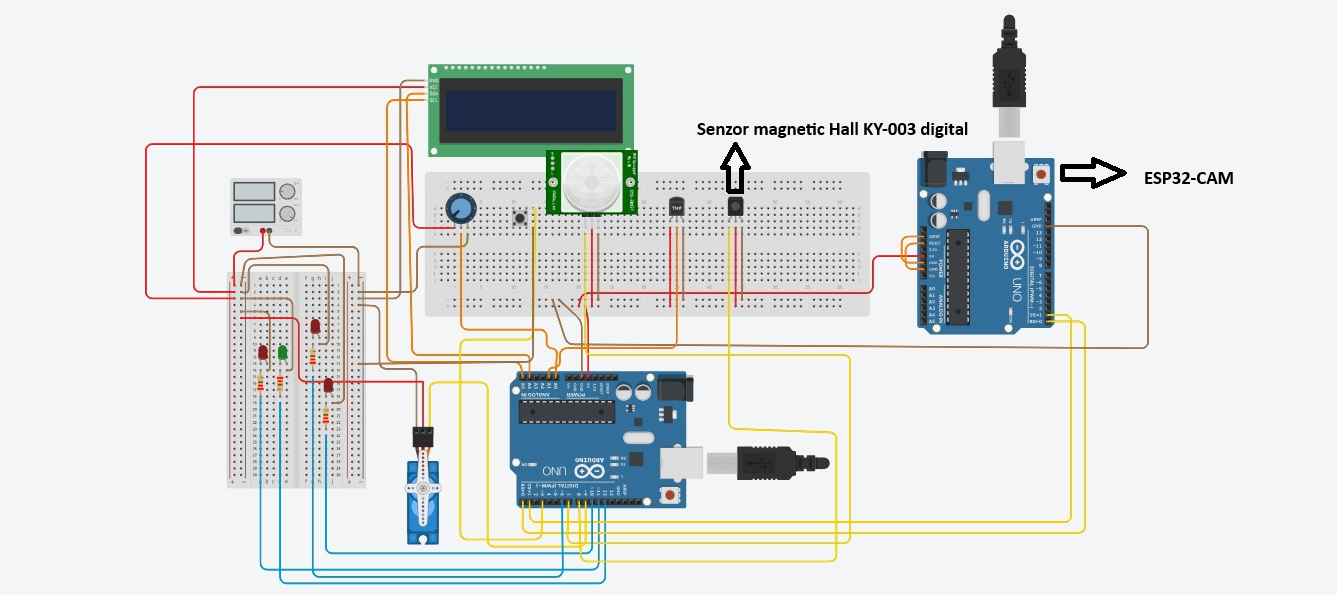
\includegraphics[width=1.0\linewidth]{SCHEMABLOC.png}
    \caption{Schema bloc}
    \label{fig:enter-label}
\end{figure}

\begin{figure}[H]
    \centering
    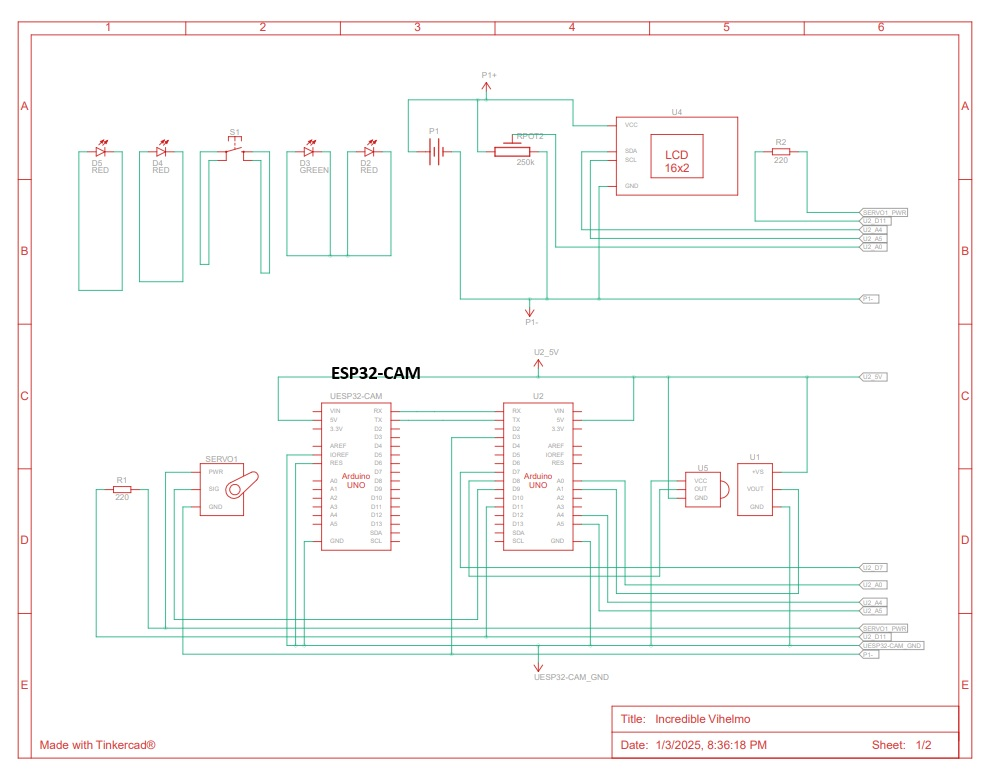
\includegraphics[width=0.8\linewidth]{SCH ELECTRICA.jpg}
    \caption{Schema electrică 1}
    \label{fig:enter-label}
\end{figure}

\begin{figure}[H]
    \centering
    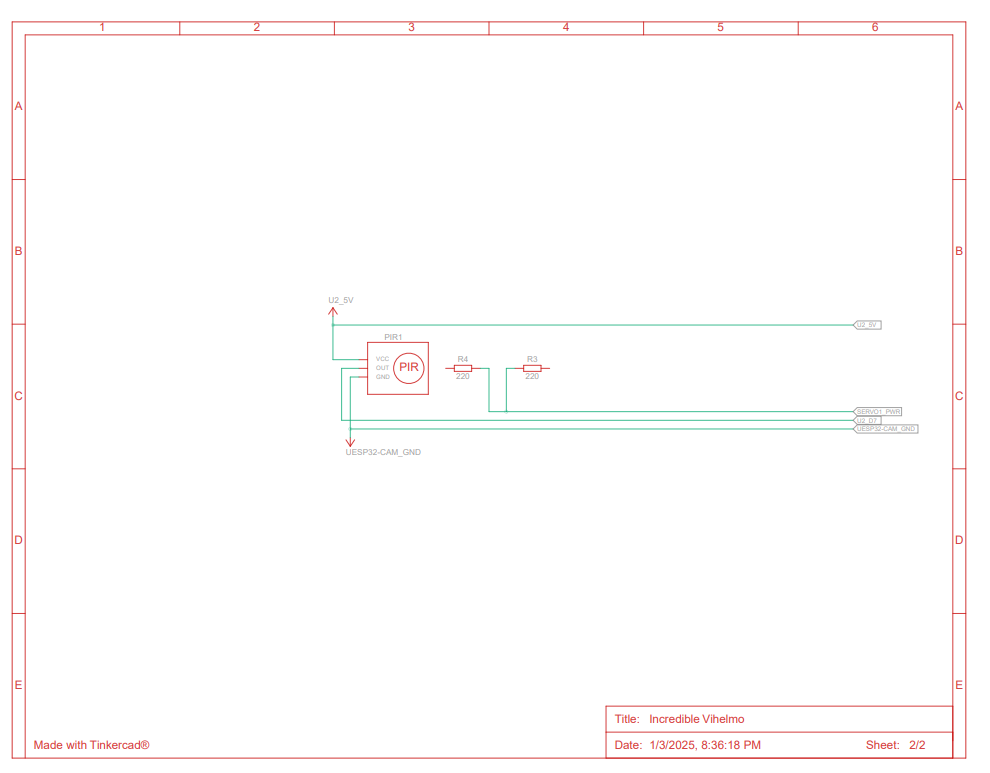
\includegraphics[width=0.8\linewidth]{SchemaElectrica2.png}
    \caption{Schema electrică 2}
    \label{fig:enter-label}
\end{figure}
\begin{figure}[H]
    \centering
    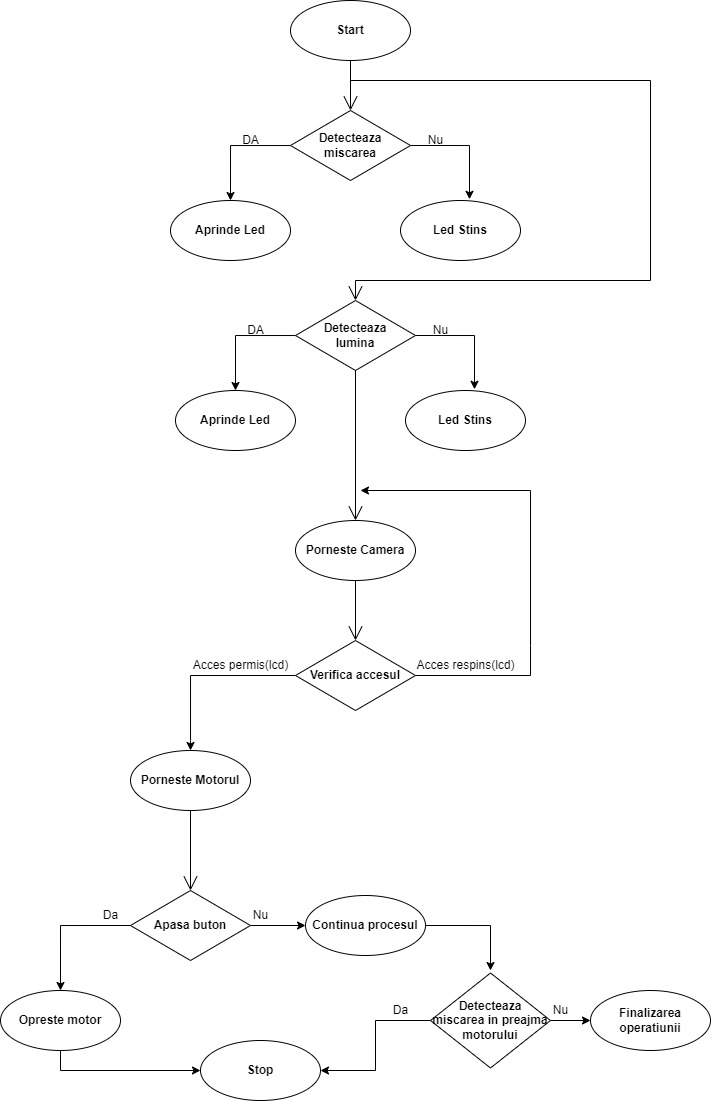
\includegraphics[width=0.8\linewidth]{Schema logica.jpg}
    \caption{Schema logică}
    \label{fig:enter-label}
\end{figure}


\chapter*{COSTURILE REALIZĂRII PRACTICE A PROIECTULUI}
\addcontentsline{toc}{chapter}{COSTURILE REALIZĂRII PRACTICE A PROIECTULUI} % Adăugăm capitolul în cuprins

Costurile pentru realizarea acestui proiect au fost împărțite pe componente hardware necesare. Mai jos este prezentat un tabel cu detalii despre fiecare componentă utilizată și prețul acestora.

\begin{table}[h!]
\centering
\resizebox{1.2\textwidth}{!}{ % Reducerea lățimii tabelului la 80% din lățimea paginii
\begin{tabular}{|c|l|c|c|}
\hline
\textbf{Nr. Crt.} & \textbf{Componentă} & \textbf{Cantitate} & \textbf{Preț unitar (RON)} \\
\hline
1  & Placa dezvoltare ESP32-CAM, Wifi, Bluetooth, OV2640 2MP & 1  & 61.32 \\
2  & Placa dezvoltare UNO, compatibila Arduino, 16U2 & 1 & 57.88 \\
3  & Senzor PIR Mini, SR602, detectie miscare, 3.3-15V & 1 & 6.43 \\
4  & Senzor magnetic Hall KY-003 digital & 1 & 2.98 \\
5  & Buton Mini 6x6x5, 4 pini & 2 & 0.36 \\
6  & Servomotor MG996R, 360 grade, 13Kg & 1 & 27.39 \\
7  & 40 Fire Dupont 30cm, Tata-Mama & 1 & 6.52 \\
8  & Rezistor 1/4W, 0.25W, 1\%, film metal - Valoare Ohm : 220 & 20 & 0.15 \\
9  & Rezistor 1/4W, 0.25W, 1\%, film metal - Valoare Ohm : 10k & 20 & 0.15 \\
10 & Rezistor 1/4W, 0.25W, 1\%, film metal - Valoare Ohm : 1k & 20 & 0.15 \\
11 & Senzor lumina ambientala TEMT6000 & 1 & 13.09 \\
12 & LED 5mm, Rosu & 2 & 0.30 \\
13 & LED 5mm, Verde & 2 & 0.30 \\
14 & Comutator magnetic Reed, N/O & 1 & 1.61 \\
15 & Potentiometru WH148, 15mm, 1K, 5K, 10K, 20K, 50K, 100K - Valoare : 50K & 3 & 2.38 \\
16 & 40 Fire Dupont 20cm, Tata-Tata & 1 & 6.51 \\
17 & LCD I2C & 1 & 30 \\
\hline
\textbf{Total comanda:} & & & \textbf{232.39} \\
\hline
\end{tabular}
}
\caption{Costurile componentelor hardware utilizate pentru proiect}
\end{table}



\chapter*{PREZENTAREA PACHETELOR SOFTWARE ȘI A LIMBAJELOR DE PROGRAMARE}
\addcontentsline{toc}{chapter}{PREZENTAREA PACHETELOR SOFTWARE } % Adăugăm capitolul în cuprins

În acest proiect, sistemul de acces controlat prin recunoaștere facială a fost realizat utilizând două componente esențiale: \textbf{Programarea pe registrii} pentru controlul hardware-ului și \textbf{OpenCV}, o librărie Python folosită pentru procesarea imaginilor și recunoașterea facială.

\subsection*{Programarea pe registrii}
\addcontentsline{toc}{subsection}{Programarea pe registrii}

În cadrul acestui proiect, o parte importantă a funcționalităților hardware a fost implementată utilizând programarea pe registrii. Această abordare permite accesul direct la componentele hardware ale microcontrolerului, oferind control total asupra operațiunilor și performanță crescută.

\textbf{Exemple de utilizare a registrilor în proiect}:
\begin{itemize}
    \item \textbf{Inițializarea și controlul protocolului I2C}: \
    Programarea pe registrii a fost utilizată pentru a comunica cu un afișaj LCD prin protocolul I2C. Funcții precum \texttt{i2c\_init}, \texttt{i2c\_start}, \texttt{i2c\_stop} și \texttt{i2c\_write} gestionează direct semnalele I2C prin manipularea registrelor dedicate (\texttt{TWSR}, \texttt{TWBR}, \texttt{TWCR}).

    \item \textbf{Controlul afișajului LCD}: \
    Registrii au fost utilizați pentru configurarea afișajului LCD și transmiterea comenzilor către acesta. De exemplu, funcția \texttt{lcd\_init} configurează afișajul folosind comenzi specifice prin I2C, iar alte funcții precum \texttt{lcd\_clear} și \texttt{lcd\_print} actualizează conținutul afișajului.

    \item \textbf{Controlul servomotorului}: \
    Registrii timer-ului hardware au fost folosiți pentru generarea unui semnal PWM precis, necesar controlului poziției servomotorului. Configurarea registrelor \texttt{TCCR1A}, \texttt{TCCR1B}, și \texttt{OCR1A} asigură mișcarea lină a servomotorului pentru deschiderea sau închiderea accesului.

    \item \textbf{Manipularea semnalelor pentru senzori și LED-uri}: \
    Registrii de intrare-ieșire (\texttt{PORTB}, \texttt{PORTD}, etc.) au fost folosiți pentru a controla LED-uri, senzori și alte componente conectate la microcontroler.
\end{itemize}

Această abordare oferă avantajul unui control foarte precis și eficient al componentelor hardware, fiind indispensabilă în proiectele în care optimizarea performanței și a resurselor este esențială.

\subsection*{OpenCV pentru recunoaștere facială}
\addcontentsline{toc}{subsection}{OpenCV pentru recunoaștere facială}

Pe partea software, librăria \textbf{OpenCV} a fost utilizată pentru procesarea imaginilor și implementarea algoritmului de recunoaștere facială. Aceasta a permis:
\begin{itemize}
    \item \textbf{Capturarea și preprocesarea imaginilor}: Imaginile primite de la ESP32-CAM au fost ajustate pentru a fi utilizate în procesul de recunoaștere.
    \item \textbf{Detecția feței}: OpenCV a fost utilizată pentru a localiza fețele în imaginile capturate.
    \item \textbf{Compararea fețelor}: Fețele detectate au fost comparate cu cele stocate în baza de date, iar rezultatele au fost transmise către microcontroler pentru a permite sau refuza accesul.
\end{itemize}

Această integrare a programării pe registrii cu OpenCV demonstrează modul în care hardware-ul și software-ul pot colabora pentru a implementa un sistem de acces performant și eficient.

\section{Fluxul General al Aplicației}
\addcontentsline{toc}{section}{Fluxul General al Aplicației} % Adăugăm secțiunea în cuprins


\subsection{Capturarea imaginii}
ESP32-CAM capturează imagini și le transmite la serverul Python folosind Wi-Fi. Aceste imagini sunt accesibile la un IP specificat de ESP32-CAM.

\subsection{Prelucrarea imaginii cu Python}
La serverul Python, librăria \texttt{\textbf{face\_recognition}} analizează imaginea capturată, detectând fețele și comparându-le cu cele din baza de date.

\subsection{Autorizarea accesului}
Dacă fața recunoscută corespunde cu una dintre fețele autorizate, Arduino primește un semnal de „PERMIS” și deschide accesul, pornind servomotorul și aprinzând LED-ul verde. Dacă nu, Arduino primește un semnal de „RESPINS” și sistemul rămâne închis.

\subsection{Controlul accesului}
Un buton de oprire permite utilizatorului să oprească complet sistemul, iar un senzor de mișcare PIR detectează mișcarea și poate activa un bliț pentru a îmbunătăți iluminarea atunci când este necesar.

\section*{Colaborarea celor două limbaje de programare}
\addcontentsline{toc}{section}{Colaborarea celor două limbaje de programare} % Adăugăm secțiunea în cuprins

Cele două limbaje de programare lucrează împreună pentru a crea un sistem de acces automatizat, bazat pe recunoașterea facială, care interacționează atât cu hardware-ul (prin Arduino), cât și cu software-ul avansat de procesare a imaginilor (prin Python).


\chapter*{Fragmente de cod sursă relevante}
\addcontentsline{toc}{chapter}{FRAGMENTE DE COD SURSĂ RELEVANTE} % Adăugăm capitolul în cuprins

\subsection{Capturarea imaginii de la ESP32-CAM}
Primul pas în procesul de recunoaștere facială este capturarea imaginii de la ESP32-CAM. Codul trimite o cerere HTTP către ESP32 pentru a obține fluxul video.

\begin{lstlisting}[caption={Capturarea imaginii de la ESP32-CAM}]
response = requests.get(ESP32_URL, timeout=5)
if response.status_code != 200:
    print("Eroare la obținerea imaginii de la ESP32.")
    continue
\end{lstlisting}

\subsection{Detectarea și Compararea Fețelor}
Aici, utilizăm librăria \texttt{face\_recognition} pentru a detecta fețele și pentru a le compara cu fețele cunoscute stocate în sistem. Dacă o față este recunoscută, se trimite un semnal către Arduino pentru a permite accesul.

\begin{lstlisting}[caption={Detectarea și compararea fețelor}]
face_locations = face_recognition.face_locations(rgb_frame)
face_encodings = face_recognition.face_encodings(rgb_frame, face_locations)

face_recognized = False
detected_name = "Necunoscut"
for face_encoding in face_encodings:
    matches = face_recognition.compare_faces(known_faces, face_encoding, tolerance=0.6)
    if True in matches:
        match_index = matches.index(True)
        detected_name = known_names[match_index]
        face_recognized = True
        break
\end{lstlisting}

\subsection{Trimiterea rezultatului către Arduino}
În funcție de rezultatul recunoașterii faciale, se trimite un semnal către Arduino pentru a permite sau respinge accesul. Dacă fața este recunoscută, se trimite un semnal de "PERMIS", iar dacă nu, se trimite "RESPINS".

\begin{lstlisting}[caption={Trimiterea rezultatului către Arduino}]
if face_recognized:
    print(f"Acces permis pentru utilizatorul: {detected_name}")
    try:
        arduino.write(b'PERMIS\n')  # Trimite "PERMIS" către Arduino
    except serial.SerialException as e:
        print(f"Eroare la scrierea în Arduino: {e}")
else:
    print("Acces respins.")
    try:
        arduino.write(b'RESPINS\n')  # Trimite "RESPINS" către Arduino
    except serial.SerialException as e:
        print(f"Eroare la scrierea în Arduino: {e}")
\end{lstlisting}

\subsection{Desenarea rezultatelor pe imagine}
Pe imaginea capturată, se adaugă un dreptunghi verde sau roșu în jurul feței, în funcție de rezultatul recunoașterii. În plus, pe imagine se va afișa un mesaj care indică dacă accesul a fost permis sau respins.

\begin{lstlisting}[caption={Desenarea rezultatelor pe imagine}]
for (top, right, bottom, left) in face_locations:
    color = (0, 255, 0) if face_recognized else (0, 0, 255)
    message = f"Acces Permis: {detected_name}" if face_recognized else "Acces Respins"
    cv2.rectangle(frame, (left, top), (right, bottom), color, 2)
    cv2.putText(frame, message, (left, top - 10), cv2.FONT_HERSHEY_SIMPLEX, 0.6, color, 2)
\end{lstlisting}

\subsection{Oprirea sistemului}
Sistemul poate fi oprit de utilizator prin apăsarea tastei 'q'. În acest caz, sistemul va trimite semnalul "RESPINS" către Arduino și va închide aplicația.

\begin{lstlisting}[caption={Oprirea sistemului}]
if cv2.waitKey(1) & 0xFF == ord('q'):
    print("Oprire sistem. Acces respins.")
    try:
        arduino.write(b'RESPINS\n')  # Trimite "RESPINS" către Arduino
    except serial.SerialException as e:
        print(f"Eroare la scrierea în Arduino: {e}")
    system_off = True
    break
\end{lstlisting}


\section{Definirea constantelor pentru LCD și I2C}
\textbf{Cod:}
\begin{lstlisting}
#define LCD_ADDR 0x27
#define LCD_CLEARDISPLAY 0x01
#define LCD_RETURNHOME 0x02
#define LCD_ENTRYMODESET 0x04
#define LCD_DISPLAYCONTROL 0x08
#define LCD_CURSORSHIFT 0x10
#define LCD_FUNCTIONSET 0x20
#define LCD_SETCGRAMADDR 0x40
#define LCD_SETDDRAMADDR 0x80

#define LCD_ENTRYRIGHT 0x00
#define LCD_ENTRYLEFT 0x02
#define LCD_ENTRYSHIFTINCREMENT 0x01
#define LCD_ENTRYSHIFTDECREMENT 0x00

#define LCD_DISPLAYON 0x04
#define LCD_DISPLAYOFF 0x00
#define LCD_CURSORON 0x02
#define LCD_CURSOROFF 0x00
#define LCD_BLINKON 0x01
#define LCD_BLINKOFF 0x00

#define LCD_8BITMODE 0x10
#define LCD_4BITMODE 0x00
#define LCD_2LINE 0x08
#define LCD_1LINE 0x00
#define LCD_5x10DOTS 0x04
#define LCD_5x8DOTS 0x00

#define LCD_BACKLIGHT 0x08
#define LCD_NOBACKLIGHT 0x00

#define En 0x04
#define Rw 0x02
#define Rs 0x01
\end{lstlisting}

\textbf{Explicație:}
\begin{itemize}
    \item Definițiile sunt utilizate pentru configurarea și controlul LCD-ului prin protocolul I2C.
    \item \texttt{LCD\_ADDR} specifică adresa I2C a LCD-ului.
    \item Alte constante definesc comenzi și moduri de operare pentru LCD, cum ar fi afișajul activ/inactiv, modul cursorului și dimensiunea afișajului.
\end{itemize}

\section{Definirea variabilelor globale și a pinilor hardware}
\textbf{Cod:}
\begin{lstlisting}
bool isAccessGranted = false;
bool isSystemOff = false;
uint8_t _displayfunction;
uint8_t _displaycontrol;
uint8_t _displaymode;
uint8_t _backlightval;

const int ledGreen = 12;
const int ledRed = 11;
const int potentiometerPin = A0;
const int buttonPin = 3;
const int pirPin = 7;
const int pirLed = 6;
#define light A1
#define ledPin 10
const int hallSensorPin = 8;
\end{lstlisting}

\textbf{Explicație:}
\begin{itemize}
    \item Variabilele globale \texttt{isAccessGranted} și \texttt{isSystemOff} controlează accesul și starea sistemului.
    \item Variabilele \texttt{\_displayfunction}, \texttt{\_displaycontrol}, \texttt{\_displaymode}, și \texttt{\_backlightval} gestionează funcțiile interne ale LCD-ului.
    \item Definirea pinilor hardware este utilizată pentru LED-uri, senzori, potențiometru și butoane.
\end{itemize}

\section{Funcții I2C pentru controlul registrilor}
\textbf{Cod:}
\begin{lstlisting}
void i2c_init() {
    TWSR = 0;
    TWBR = ((F_CPU/100000L)-16)/2;
    TWCR = (1<<TWEN);
}

void i2c_start() {
    TWCR = (1<<TWINT)|(1<<TWSTA)|(1<<TWEN);
    while (!(TWCR & (1<<TWINT)));
}

void i2c_stop() {
    TWCR = (1<<TWINT)|(1<<TWEN)|(1<<TWSTO);
    while(TWCR & (1<<TWSTO));
}

void i2c_write(uint8_t data) {
    TWDR = data;
    TWCR = (1<<TWINT)|(1<<TWEN);
    while (!(TWCR & (1<<TWINT)));
}

void i2c_send_byte(uint8_t addr, uint8_t data) {
    i2c_start();
    i2c_write(addr<<1);
    i2c_write(data);
    i2c_stop();
}
\end{lstlisting}

\textbf{Explicație:}
\begin{itemize}
    \item Funcțiile initializează și controlează comunicarea I2C.
    \item \texttt{i2c\_init()} configurează viteza și activarea magistralei I2C.
    \item \texttt{i2c\_start()} și \texttt{i2c\_stop()} gestionează semnalele de început și sfârșit pentru comunicare.
    \item \texttt{i2c\_write()} și \texttt{i2c\_send\_byte()} trimit date către dispozitivele conectate.
\end{itemize}

\section{Inițializarea și funcționarea LCD-ului}
\textbf{Cod:}
\begin{lstlisting}
void lcd_init() {
    i2c_init();
    _displayfunction = LCD_4BITMODE | LCD_2LINE | LCD_5x8DOTS;
    _backlightval = LCD_BACKLIGHT;

    delay(50);
    expanderWrite(0);
    delay(1000);

    write4bits(0x03 << 4);
    delayMicroseconds(4500);
    write4bits(0x03 << 4);
    delayMicroseconds(4500);
    write4bits(0x03 << 4);
    delayMicroseconds(150);
    write4bits(0x02 << 4);

    command(LCD_FUNCTIONSET | _displayfunction);

    _displaycontrol = LCD_DISPLAYON | LCD_CURSOROFF | LCD_BLINKOFF;
    command(LCD_DISPLAYCONTROL | _displaycontrol);

    lcd_clear();

    _displaymode = LCD_ENTRYLEFT | LCD_ENTRYSHIFTDECREMENT;
    command(LCD_ENTRYMODESET | _displaymode);

    command(LCD_RETURNHOME);
    delay(2);
}
\end{lstlisting}

\textbf{Explicație:}
\begin{itemize}
    \item Funcția \texttt{lcd\_init()} inițializează LCD-ul și configurările sale, precum modul de afișare și iluminarea de fundal.
    \item \texttt{expanderWrite()} și \texttt{write4bits()} sunt utilizate pentru a trimite date către LCD folosind I2C.
\end{itemize}

\section{Funcții principale din \texttt{setup()} și \texttt{loop()}}
\textbf{Cod:}
\begin{lstlisting}
void setup() {
    Serial.begin(115200);

    pinMode(hallSensorPin, INPUT);

    lcd_init();
    lcd_print("Sistem pornit");
    delay(2000);
    lcd_clear();

    Serial.println("Sistem Arduino pornit. Astept mesaje...");
}

void loop() {
    if (isSystemOff) {
        lcd_clear();
        lcd_print("Sistem oprit");
        while(1);
    }

    if (Serial.available() > 0) {
        String message = Serial.readStringUntil('\n');
        if (message == "PERMIS") {
            isAccessGranted = true;
            lcd_clear();
            lcd_print("Acces permis");
        } else if (message == "RESPINS") {
            isAccessGranted = false;
            lcd_clear();
            lcd_print("Acces respins");
        } else {
            lcd_clear();
            lcd_print("Mesaj necunoscut");
        }
    }
}
\end{lstlisting}

\textbf{Explicație:}
\begin{itemize}
    \item \texttt{setup()} configurează hardware-ul și afișează mesajul de pornire.
    \item \texttt{loop()} gestionează evenimentele principale, inclusiv mesaje de la serial, senzorii PIR și Hall, și controlul LED-urilor.
\end{itemize}


\section{Configurarea conexiunii WiFi}
Parametrii pentru rețeaua WiFi (SSID și parola) sunt specificați prin intermediul variabilelor globale. Acest lucru permite conectarea automată la o rețea specificată.

\begin{lstlisting}[language=C, caption=Configurarea rețelei WiFi]
const char* ssid = "DIGI-n3p2";
const char* password = "4tw88U3F";
\end{lstlisting}

\section{Configurarea camerei}
Funcția \texttt{setup()} inițializează camera folosind structura de mai jos.

\begin{lstlisting}[language=C, caption=Inițializarea configurației camerei]
camera_config_t config;
config.ledc_channel = LEDC_CHANNEL_0;
config.ledc_timer = LEDC_TIMER_0;
config.pin_d0 = Y2_GPIO_NUM;
config.pin_d1 = Y3_GPIO_NUM;
...
config.xclk_freq_hz = 20000000;
config.frame_size = FRAMESIZE_UXGA;
config.pixel_format = PIXFORMAT_JPEG; // for streaming
\end{lstlisting}

Pentru optimizarea performanței, dacă \texttt{PSRAM} este detectat, calitatea JPEG este îmbunătățită și numărul bufferelor este mărit. Dacă nu este disponibil \texttt{PSRAM}, dimensiunea cadrului este redusă.

\begin{lstlisting}[language=C, caption=Optimizare pentru PSRAM]
if(psramFound()){
config.jpeg_quality = 10;
config.fb_count = 2;
} else {
config.frame_size = FRAMESIZE_SVGA;
config.fb_location = CAMERA_FB_IN_DRAM;
}
\end{lstlisting}

\section{Conectarea la WiFi și pornirea serverului web}
După inițializarea camerei, dispozitivul se conectează la rețeaua WiFi utilizând funcția \texttt{WiFi.begin()}. După conectare, un server web este pornit pentru streaming video.

\begin{lstlisting}[language=C, caption=Conectarea la WiFi și inițializarea serverului]
WiFi.begin(ssid, password);
while (WiFi.status() != WL_CONNECTED) {
delay(500);
Serial.print(".");
}
Serial.println("WiFi connected");
startCameraServer();
\end{lstlisting}

Adresa IP locală a dispozitivului este afișată în consolă pentru accesul la interfața web:

\begin{lstlisting}[language=C, caption=Afișarea adresei IP]
Serial.print("Camera Ready! Use 'http://");
Serial.print(WiFi.localIP());
Serial.println("' to connect");
\end{lstlisting}

\section{Bucla principală}
Bucla principală \texttt{loop()} nu conține logică adițională, deoarece serverul web gestionează toate operațiunile. O întârziere este folosită pentru a preveni rularea continuă inutilă.

\begin{lstlisting}[language=C, caption=Bucla principală]
void loop() {
delay(10000);
}
\end{lstlisting}

\section{Concluzii}
Acest cod oferă un punct de plecare pentru dezvoltarea aplicațiilor bazate pe camere ESP32, permițând utilizatorilor să ajusteze configurațiile în funcție de cerințele hardware și aplicație.


\section{Statistici legate de numărul de linii de cod și timpul necesar dezvoltării}

Pentru a evalua complexitatea proiectului și timpul necesar pentru dezvoltarea acestuia, vom analiza numărul total de linii de cod din cele două module principale ale proiectului: programul pentru microcontroler și programul pentru recunoașterea facială.

\subsection{Cod pentru microcontroler (Arduino)}
\begin{itemize}
    \item \textbf{Număr total de linii}: 253
    \item \textbf{Funcții principale}:
    \begin{itemize}
        \item Funcții pentru inițializarea și operarea afișajului LCD.
        \item Funcții pentru controlul senzorilor și dispozitivelor (PIR, Hall, buton, LED-uri, servomotor).
        \item Comunicare prin serial și procesarea comenzilor primite.
    \end{itemize}
    \item \textbf{Timp estimat pentru dezvoltare și testare}: Aproximativ \textbf{20-25 ore} (inclusiv debug).
\end{itemize}

\subsection{Cod pentru recunoaștere facială (Python)}
\begin{itemize}
    \item \textbf{Număr total de linii}: 107
    \item \textbf{Funcții principale}:
    \begin{itemize}
        \item Inițializarea și procesarea imaginii capturate de ESP32-CAM.
        \item Recunoașterea facială utilizând biblioteca \texttt{face\_recognition}.
        \item Comunicarea cu Arduino pentru transmiterea rezultatelor.
    \end{itemize}
    \item \textbf{Timp estimat pentru dezvoltare și testare}: Aproximativ \textbf{15-20 ore} (inclusiv integrarea cu ESP32-CAM și Arduino).
\end{itemize}

\subsection{Cod pentru conexiunea Esp32-Cam(Arduino)}
\begin{itemize}
\item \textbf{Număr total de linii}: 165
    \item \textbf{Funcții principale}:
    \begin{itemize}
        \item setup(): Configurează camera (inclusiv pinii și setările de imagine).
        \item loop(): Execută o buclă pasivă (doar întârziere de 10 secunde).
        \item startCameraServer(): Funcția este declarată, dar codul său nu este inclus în fragment. (Probabil gestionează serverul web pentru transmiterea video).
    \end{itemize}
   \item \textbf{Timp estimat pentru dezvoltare și testare}: Aproximativ \textbf{15-20 ore}.
\end{itemize}


\section{Interfața grafică a aplicației}
\begin{figure}[H]
    \centering
    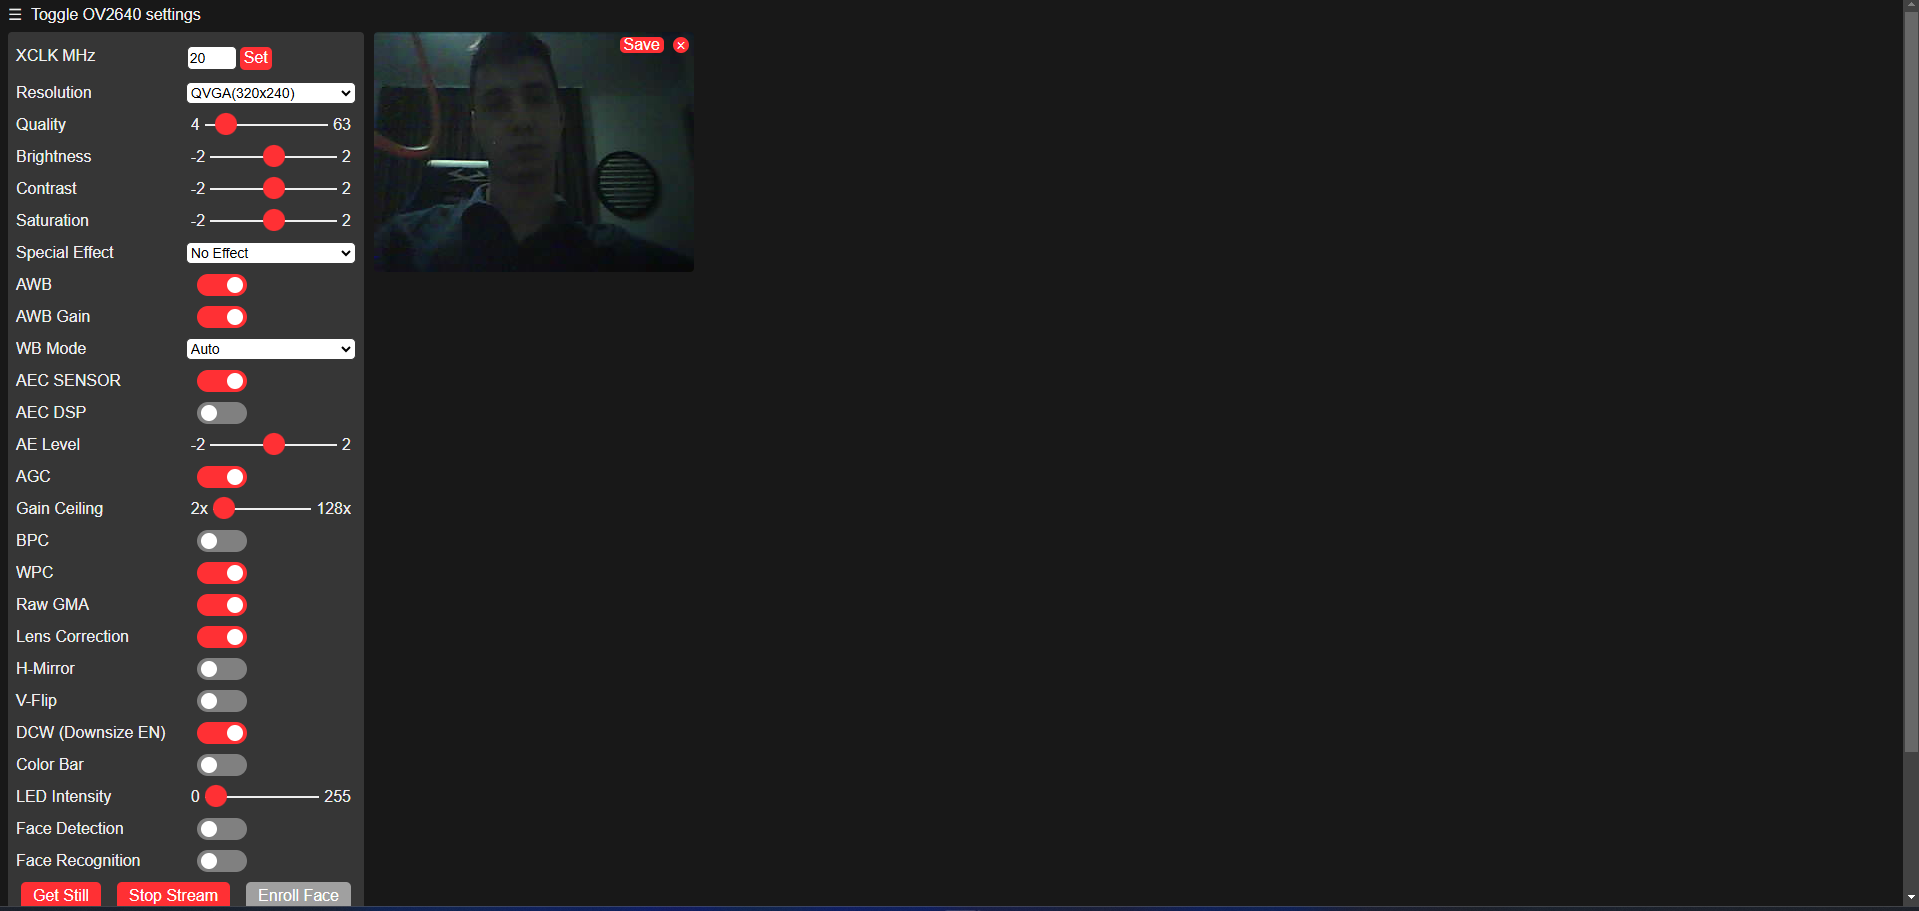
\includegraphics[width=1.0\linewidth]{interfata grafica.png}
    \caption{Interfața grafică}
    \label{fig:enter-label}
\end{figure}
Această interfață grafică este utilizată pentru configurarea și controlul unei camere ESP32, permițând utilizatorului să ajusteze diferite setări și să monitorizeze fluxul video în timp real. Este împărțită în două secțiuni principale:

\begin{itemize}
    \item \textbf{Setări Configurabile}: Permite ajustarea parametrilor camerei, cum ar fi rezoluția, luminozitatea, contrastul, saturația și multe altele.
    \item \textbf{Previzualizare Video}: Afișează un flux video live de la cameră, cu opțiuni pentru capturarea imaginilor statice.
\end{itemize}

\section{Detalii ale Interfeței}
\begin{itemize}
    \item \textbf{Setări ESP32}:
    \begin{itemize}
        \item \textbf{XCLK MHz}: Frecvența semnalului de ceas pentru cameră.
        \item \textbf{Resolution}: Selectarea rezoluției video (ex: QVGA).
        \item \textbf{Quality}: Reglarea calității imaginii.
        \item \textbf{Brightness, Contrast, Saturation}: Ajustări pentru optimizarea imaginii.
        \item \textbf{Special Effect}: Aplicarea de efecte vizuale speciale (ex: monocrom).
        
    \end{itemize}

\end{itemize}


\chapter*{PREZENTAREA MONTAJULUI REALIZAT}
\begin{figure}[H]
    \centering
    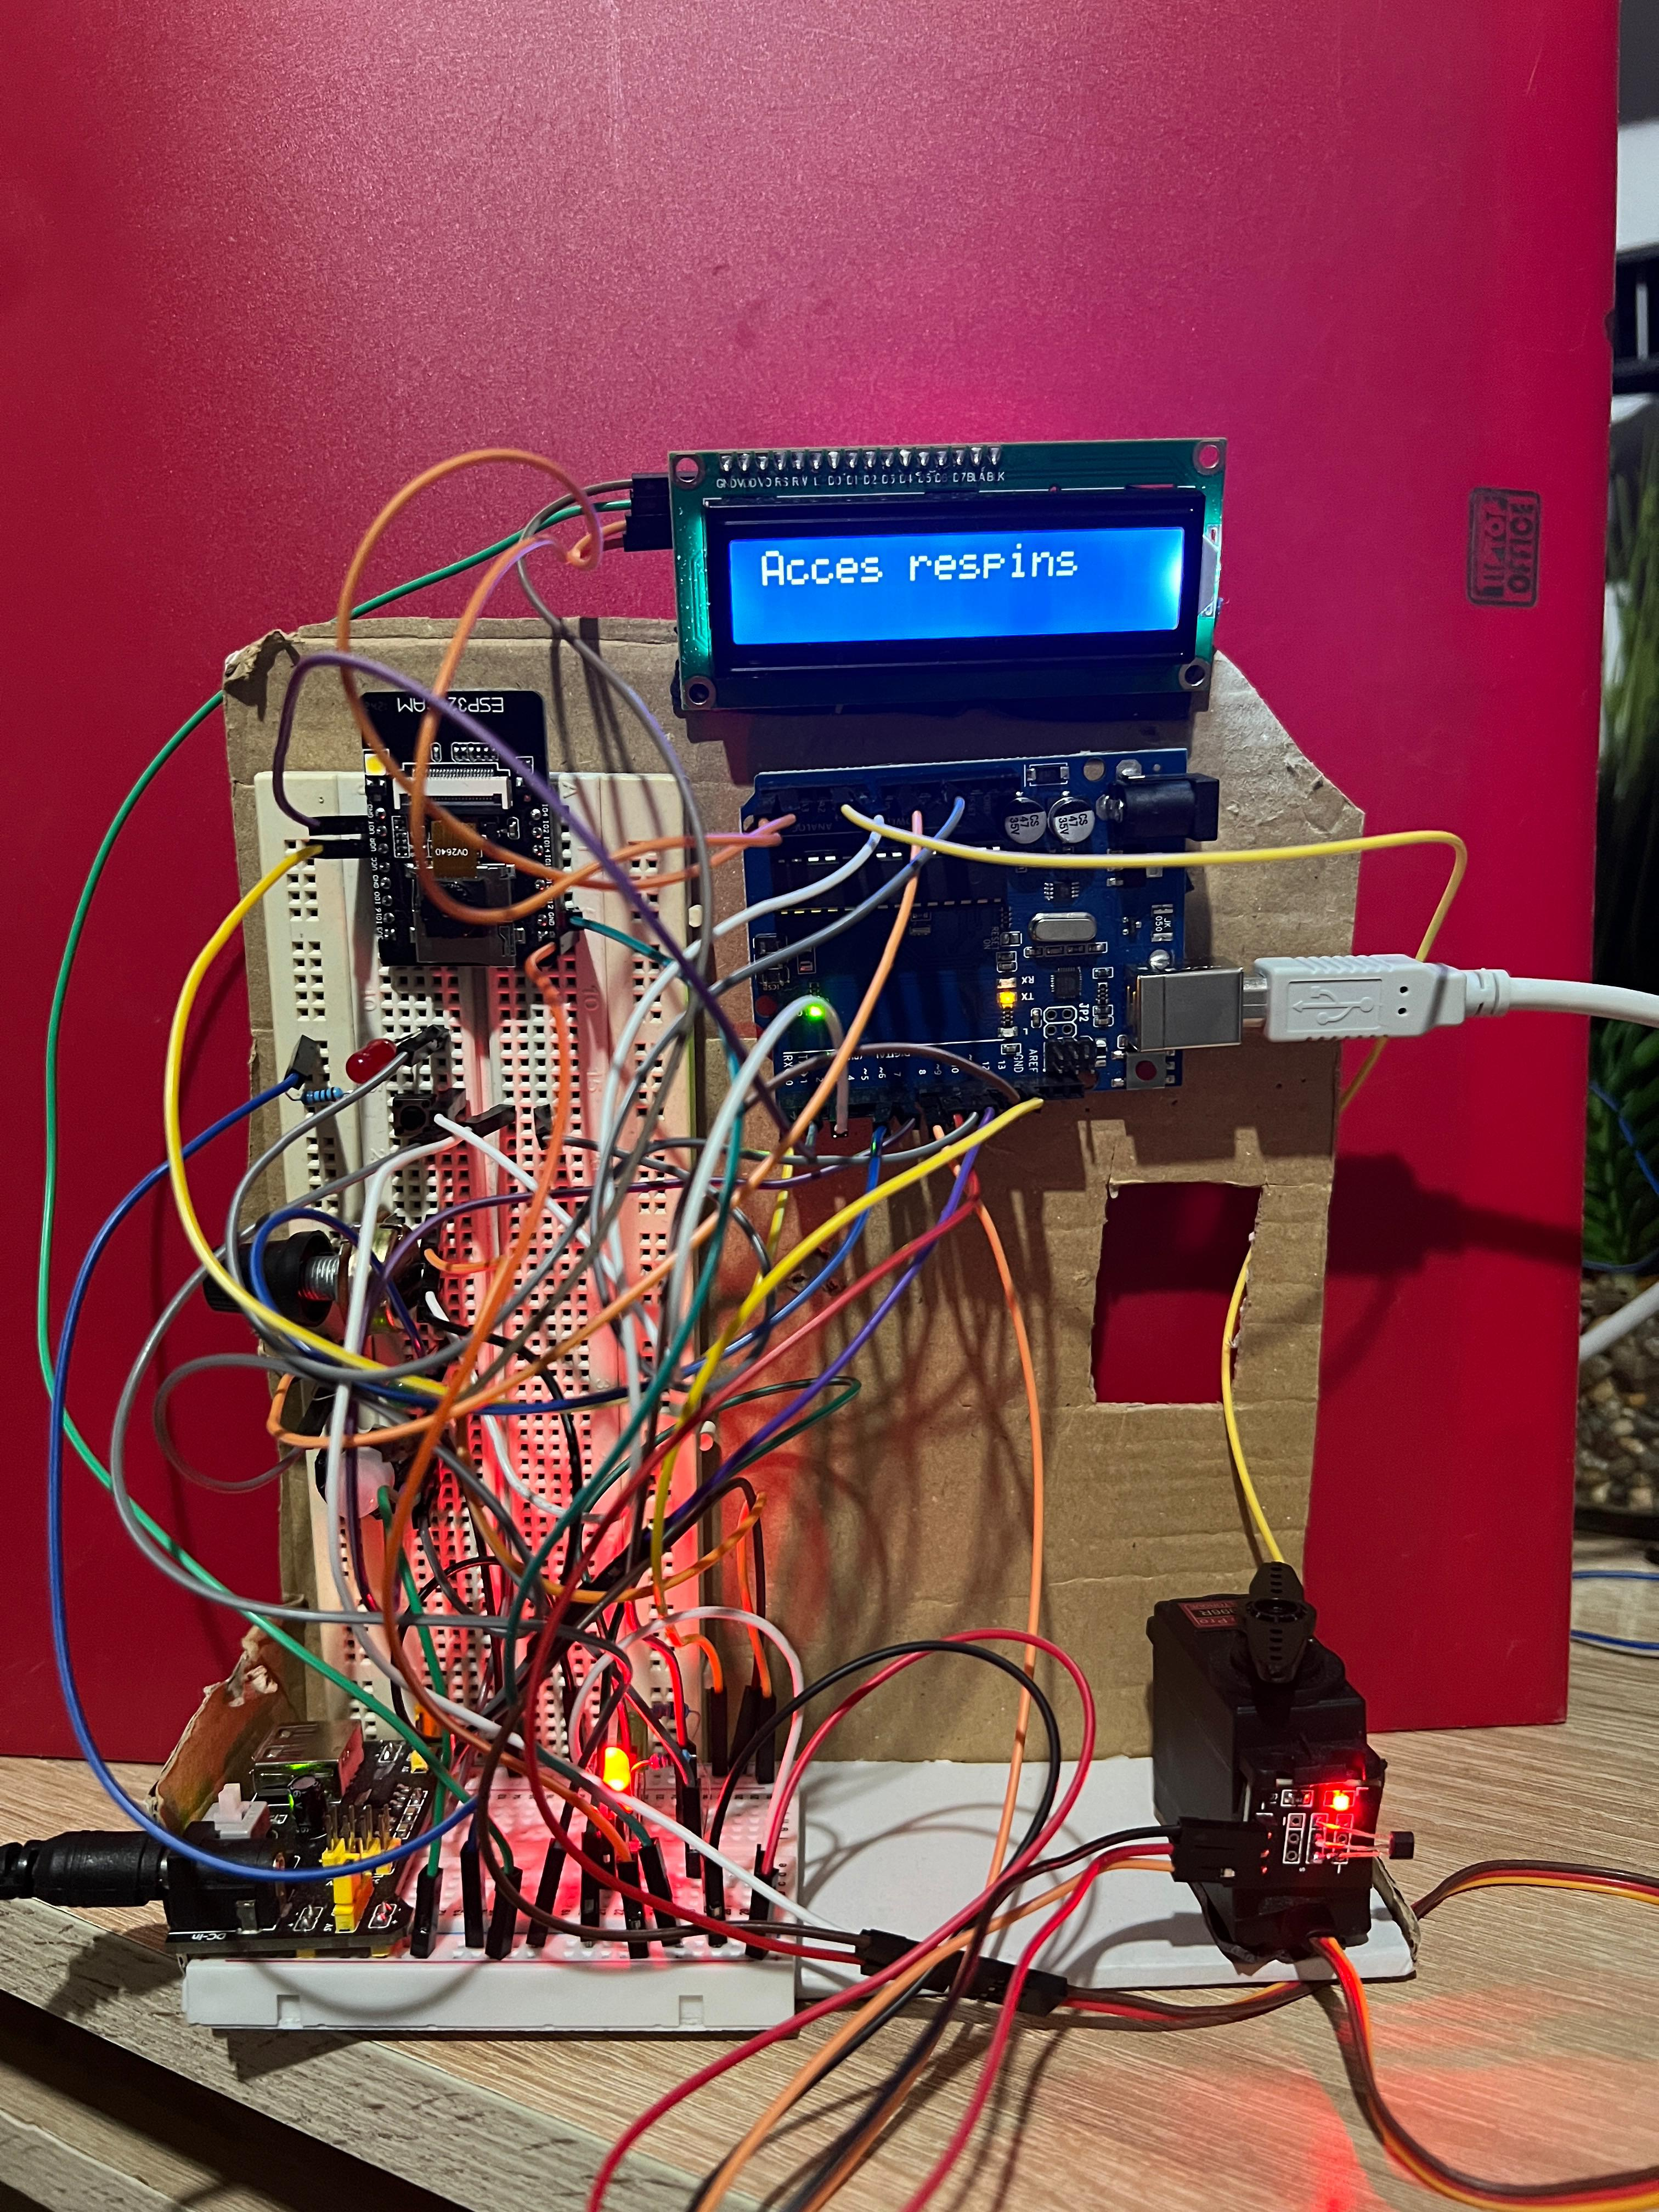
\includegraphics[width=0.7\linewidth]{montajul propriu-zis.jpg}
    \caption{Montajul propriu-zis}
    \label{fig:enter-label}
\end{figure}
În această secțiune, sunt prezentate în detaliu componentele hardware utilizate în cadrul proiectului, evidențiind fiecare componentă individual. După descrierea acestora, este ilustrat modul în care acestea au fost integrate pentru realizarea montajului final.

\section{Descrierea montajului}

Montajul prezentat include următoarele componente:
\begin{itemize}
    \item \textbf{Arduino Uno}: Microcontroler principal, care controlează logica și semnalele sistemului.
    \item \textbf{Modul ESP32-CAM}: Modul Wi-Fi cu cameră integrată, utilizat pentru captură video și transmiterea datelor.
    \item \textbf{LCD}: Afișează informații text sau date generate de sistem.
    \item \textbf{Potentiometru}: Permite ajustarea contrastului sau a altor parametri.
    \item \textbf{Servomotor}: Realizează mișcări precise, controlat de Arduino.
    \item \textbf{LED-uri}: Două LED-uri, unul roșu și unul verde, pentru semnalizare și încă două leduri, unul pentru senzorul de lumină si unul pentru senzorul de mișcare.
    \item \textbf{Rezistențe}: Protejează LED-urile prin limitarea curentului.
    \item \textbf{Placă de dezvoltare (Breadboard)}: Asigură conectarea componentelor fără lipire.
    \item \textbf{Fire de conectare}: Conectează componentele, utilizând culori diferite pentru semnal, alimentare și masă
    \item \textbf{Buton:} Odată ce este apăsat, oprește funcționarea circuitului.
     \item \textbf{Senzor lumina ambientala TEMT6000:} Ajută la detectarea luminii din incapere, iar in cazul in care este scăzută, se aprinde un led roșu.
    
\end{itemize}

\chapter*{PERFORMANȚE}
\addcontentsline{toc}{chapter}{PERFORMANȚE} % Adăugăm capitolul în cuprins
Performanțele sistemului nostru au fost evaluate pe baza mai multor criterii esențiale: eficiența recunoașterii, promptitudinea răspunsului motorului servo și stabilitatea generală în timpul utilizării continue.

\section{Eficiența recunoașterii}
Sistemul este capabil să detecteze și să proceseze imagini faciale cu un grad ridicat de acuratețe, oferind rezultate consistente chiar și în condiții de luminozitate variabilă.

\section{Promptitudinea răspunsului motorului servo}
Motorul servo răspunde rapid la comenzile primite, permițând deschiderea și închiderea precisă a mecanismelor asociate fără întârzieri semnificative.

\section{Stabilitatea sistemului}
Sistemul a fost testat pentru rulare continuă pe perioade extinse, demonstrând fiabilitate și rezistență, fără întreruperi sau pierderi de performanță. Toate componentele hardware și software au funcționat în mod sincronizat și stabil.

\section{Rezumatul performanțelor}


\begin{table}[H]
    \centering
    \begin{tabular}{|l|c|}
        \hline
        \textbf{Parametru} & \textbf{Performanță} \\ \hline
        Eficiența recunoașterii faciale & Ridicată \\ \hline
        Răspunsul motorului servo & Prompt \\ \hline
        Stabilitatea sistemului & Consistentă \\ \hline
    \end{tabular}
    \caption{Performanțele sistemului de acces}
    \label{tab:performante}
\end{table}


\chapter*{CONCLUZII}
\addcontentsline{toc}{chapter}{CONCLUZII} % Adăugăm capitolul în cuprins

Proiectul realizat reprezintă o integrare reușită între tehnologia hardware și software, demonstrând modul în care componentele electronice pot fi coordonate pentru a obține un sistem funcțional și eficient. Utilizarea platformei Arduino a oferit o bază solidă pentru gestionarea și controlul componentelor hardware, cum ar fi LED-urile, servomotorul, modulul ESP32-CAM și afișajul LCD, fiecare contribuind la funcționalitatea generală a sistemului.

De asemenea, Python a fost esențial în partea de prelucrare a imaginilor și pentru realizarea unor funcționalități avansate. Această abordare a permis integrarea facilă a modulului ESP32-CAM pentru captură și procesare de imagini, facilitând transmiterea datelor în timp real și posibilitatea extinderii proiectului către aplicații IoT sau de monitorizare inteligentă. Limbajul Python, prin bibliotecile sale puternice, cum ar fi OpenCV, a permis manipularea eficientă a imaginilor și interpretarea datelor primite.

Succesul acestui proiect subliniază importanța combinării cunoștințelor teoretice cu abilitățile practice de implementare. Integrarea componentelor hardware cu soluții software a oferit o experiență completă, învățându-ne cum să trecem de la un concept inițial la un produs final funcțional. În plus, procesul de realizare a montajului și programarea interfeței au evidențiat cât de importantă este planificarea și organizarea în dezvoltarea unui sistem complex.

Acest proiect deschide numeroase oportunități pentru aplicații viitoare, cum ar fi automatizări inteligente, sisteme de securitate sau proiecte educaționale. Combinarea tehnologiilor utilizate - Arduino, ESP32-CAM și Python - demonstrează că soluțiile inovatoare pot fi realizate cu resurse accesibile și un spirit creativ. În ansamblu, rezultatul obținut constituie o dovadă a progresului tehnologic care poate fi realizat prin interdisciplinaritate și muncă de echipă.

\chapter*{BIBLIOGRAFIE}
\addcontentsline{toc}{chapter}{BIBLIOGRAFIE} % Adăugăm capitolul în cuprins

\begin{enumerate}
    \item Documentația oficială Arduino. \emph{Pagina produsului Arduino Uno}. [Online]. Disponibil la: 
    \url{https://www.arduino.cc/}

    \item Ghid ESP32-CAM. \emph{Introducere în utilizarea ESP32-CAM}. [Online]. Disponibil la: 
    \url{https://randomnerdtutorials.com/esp32-cam/}

    \item Bradski, G. \emph{Învățarea OpenCV: Viziune artificială cu biblioteca OpenCV}. O'Reilly Media, 2008.

    \item Rowan, M. \emph{Proiecte IoT cu Arduino și ESP32}. Packt Publishing, 2021.

    \item Adafruit. \emph{Ghid pentru afișaje LCD cu caractere}. [Online]. Disponibil la: 
    \url{https://learn.adafruit.com/character-lcds}
\end{enumerate}


\chapter*{ANEXĂ - COD SURSĂ}
\addcontentsline{toc}{chapter}{ANEXĂ - COD SURSĂ}
\section{COD ARDUINO}
\begin{lstlisting}
#define LCD_ADDR 0x27 // Adresa I2C a LCD-ului, configurabila pe hardware prin jumperi
#define LCD_CLEARDISPLAY 0x01 // Comanda pentru curatarea ecranului LCD
#define LCD_RETURNHOME 0x02 // Comanda pentru repozitionarea cursorului la pozitia initiala
#define LCD_ENTRYMODESET 0x04 // Seteaza modul de scriere a datelor, adica directia
#define LCD_DISPLAYCONTROL 0x08 // Controleaza afisajul (pornire/oprire, cursor)
#define LCD_CURSORSHIFT 0x10 // Controleaza mutarea cursorului sau scroll-ul
#define LCD_FUNCTIONSET 0x20 // Seteaza modul de operare al LCD-ului (biti, linii, matrice)
#define LCD_SETCGRAMADDR 0x40 // Seteaza adresa pentru memorie CGRAM (caractere custom)
#define LCD_SETDDRAMADDR 0x80 // Seteaza adresa pentru memorie DDRAM (afisaj normal)

// Optiuni pentru modul de intrare al LCD-ului
#define LCD_ENTRYRIGHT 0x00 // Textul este scris de la dreapta la stanga
#define LCD_ENTRYLEFT 0x02 // Textul este scris de la stanga la dreapta (mod implicit)
#define LCD_ENTRYSHIFTINCREMENT 0x01 // Seteaza cursorul sa se mute automat la urmatoarea pozitie
#define LCD_ENTRYSHIFTDECREMENT 0x00 // Cursorul ramane pe aceeasi pozitie dupa scriere

// Optiuni pentru controlul afisajului LCD
#define LCD_DISPLAYON 0x04 // Porneste afisajul
#define LCD_DISPLAYOFF 0x00 // Opreste afisajul
#define LCD_CURSORON 0x02 // Porneste cursorul vizibil
#define LCD_CURSOROFF 0x00 // Opreste cursorul vizibil
#define LCD_BLINKON 0x01 // Cursorul clipeste
#define LCD_BLINKOFF 0x00 // Cursorul nu clipeste

// Optiuni pentru modul de operare al LCD-ului
#define LCD_8BITMODE 0x10 // Modul 8-biti
#define LCD_4BITMODE 0x00 // Modul 4-biti, utilizat in proiect
#define LCD_2LINE 0x08 // Doua linii active
#define LCD_1LINE 0x00 // O singura linie activa
#define LCD_5x10DOTS 0x04 // Matrice caractere 5x10
#define LCD_5x8DOTS 0x00 // Matrice caractere 5x8, utilizat in proiect

// Controlul backlight-ului
#define LCD_BACKLIGHT 0x08 // Porneste backlight-ul
#define LCD_NOBACKLIGHT 0x00 // Opreste backlight-ul

// Controlul pinilor LCD
#define En 0x04 // Enable bit - activeaza semnalele pentru scriere
#define Rw 0x02 // Read/Write bit - selecteaza scrierea sau citirea
#define Rs 0x01 // Register Select bit - selecteaza datele sau comanda

// Variabile globale pentru controlul afisajului si sistemului
bool isAccessGranted = false; // Variabila care indica daca accesul este permis
bool isSystemOff = false; // Variabila care indica daca sistemul este oprit
uint8_t _displayfunction; // Configuratia functiilor afisajului
uint8_t _displaycontrol; // Starea actuala a controlului afisajului
uint8_t _displaymode; // Modul curent de scriere pe LCD
uint8_t _backlightval; // Starea actuala a backlight-ului

// Pini hardware utilizati in sistem
const int ledGreen = 12; // LED verde pentru indicarea accesului permis
const int ledRed = 11; // LED rosu pentru acces respins
const int potentiometerPin = A0; // Pinul potentiometrului pentru ajustari
const int buttonPin = 3; // Pinul butonului pentru oprirea sistemului
const int pirPin = 7; // Pinul senzorului PIR pentru detectie de miscare
const int pirLed = 6; // LED asociat senzorului PIR
#define light A1 // Pinul senzorului de lumina
#define ledPin 10 // Pinul pentru LED-ul care sesizeaza lumina slaba
const int hallSensorPin = 8; // Pinul pentru senzorul Hall

// Initializarea magistralei I2C
void i2c_init() {
    // TWSR (TWI Status Register): Seteaza prescaler-ul la 1
    // TWSR contine bitii TWPS1 si TWPS0 pentru a seta prescaler-ul folosit in calculul frecventei I2C
    // Valoarea 0 pentru TWPS1 si TWPS0 (TWSR = 0) corespunde unui prescaler de 1
    TWSR = 0;
    
    // Formula pentru calculul frecventei de ceas a magistralei I2C:
    // SCL_freq = F_CPU / (16 + 2 * TWBR * prescaler)
    // TWBR (TWI Bit Rate Register) seteaza rata de transfer a bitilor
    // Pentru un ceas de 16 MHz si o frecventa dorita de 100 kHz, TWBR este calculat astfel:
    TWBR = ((F_CPU / 100000L) - 16) / 2;

    // TWCR (TWI Control Register): Activeaza interfata TWI (Two-Wire Interface)
    // Bitul TWEN (TWI Enable) este setat pentru a activa hardware-ul I2C
    
    TWCR = (1 << TWEN);
}


// Trimite un semnal START pe magistrala I2C
void i2c_start() {
    // TWCR: Seteaza bitul TWSTA pentru a genera o conditie START
    // TWINT: Este setat pentru a incepe operatia si va fi resetat automat cand operatia este completata
    TWCR = (1 << TWINT) | (1 << TWSTA) | (1 << TWEN);

    // Asteapta pana cand TWINT este resetat automat, semnalizand finalizarea operatiei START
    while (!(TWCR & (1 << TWINT)));
}
// Trimite un semnal STOP pe magistrala I2C
void i2c_stop() {
    // TWCR: Seteaza bitul TWSTO pentru a genera o conditie STOP
    // TWEN: Ramane activat pentru a permite operarea interfetei TWI
    TWCR = (1 << TWINT) | (1 << TWEN) | (1 << TWSTO);

    // Asteapta pana cand TWSTO este resetat, indicand finalizarea operatiei STOP
    while (TWCR & (1 << TWSTO));
}

// Scrie un byte pe magistrala I2C
void i2c_write(uint8_t data) {
    // TWDR (TWI Data Register): Incarca datele ce urmeaza sa fie transmise
    TWDR = data;

    // TWCR: Initiaza transmisia setand bitul TWINT si activand interfata TWI
    TWCR = (1 << TWINT) | (1 << TWEN);

    // Asteapta pana cand TWINT este resetat, indicand finalizarea transmisiei
    while (!(TWCR & (1 << TWINT)));
}

// Trimite un byte catre un dispozitiv I2C specificat prin adresa
void i2c_send_byte(uint8_t addr, uint8_t data) {
    // Trimite semnalul START pentru a incepe transmisia
    i2c_start();

    // Trimite adresa dispozitivului cu bitul de scriere (LSB = 0)
    i2c_write(addr << 1);

    // Trimite byte-ul de date catre dispozitiv
    i2c_write(data);

    // Trimite semnalul STOP pentru a incheia transmisia
    i2c_stop();
}

// Functie pentru scrierea pe expanderul I2C al LCD-ului
void expanderWrite(uint8_t data) {
    // Trimite datele catre adresa I2C a expanderului, combinand datele cu valoarea curenta a backlight-ului
    i2c_send_byte(LCD_ADDR, data | _backlightval);
}

// Functie pentru generarea unui puls Enable pentru LCD
void pulseEnable(uint8_t data) {
    // Activeaza bitul Enable al expanderului pentru a incepe scrierea datelor pe LCD
    expanderWrite(data | En);
    delayMicroseconds(1);
    // dezactiveaza bitul enable al expanderului pentru a finaliza operatia
    expanderWrite(data & ~En);
    delayMicroseconds(50);
}

// Scrie pe 4 biti in LCD (folosind expanderul I2C
void write4bits(uint8_t value) {
    // Trimite nibble-ul catre expander
    expanderWrite(value);

    // Genereaza un puls Enable pentru a valida datele trimise
    pulseEnable(value);
}

void send(uint8_t value, uint8_t mode) {
    // Extrage nibble-ul superior al datelor
    uint8_t highnib = value & 0xF0;
    
    // Extrage nibble-ul inferior al datelor
    uint8_t lownib = (value << 4) & 0xF0;
    
    // Scrie nibble-ul superior si inferior catre LCD, utilizand modul specificat
    write4bits(highnib | mode);
    write4bits(lownib | mode);
}

// Trimite o comanda catre LCD
void command(uint8_t value) {
    // Trimite valoarea catre LCD in modul comanda (mode = 0)
    send(value, 0);
}

void write(uint8_t value) {
    send(value, Rs);
}

// Functie pentru initializarea LCD-ului
void lcd_init() {
    // Initializeaza magistrala I2C pentru comunicatia cu LCD-ul
    i2c_init();

    // Configuratia initiala a afisajului: modul 4 biti, 2 linii, caractere 5x8 puncte
    _displayfunction = LCD_4BITMODE | LCD_2LINE | LCD_5x8DOTS;

    // Activeaza backlight-ul LCD-ului
    _backlightval = LCD_BACKLIGHT;

    delay(50); // Pauza pentru stabilizarea initiala a LCD-ului
    expanderWrite(0); // Reseteaza expanderul
    delay(1000); // Pauza mai lunga pentru resetare

    // Secventa specifica pentru initializarea in modul 4 biti
    write4bits(0x03 << 4);
    delayMicroseconds(4500);
    write4bits(0x03 << 4);
    delayMicroseconds(4500);
    write4bits(0x03 << 4);
    delayMicroseconds(150);
    write4bits(0x02 << 4);

    // Configureaza functiile de baza ale LCD-ului
    command(LCD_FUNCTIONSET | _displayfunction);

    // Activeaza afisajul, fara cursor sau clipire
    _displaycontrol = LCD_DISPLAYON | LCD_CURSOROFF | LCD_BLINKOFF;
    command(LCD_DISPLAYCONTROL | _displaycontrol);

    // Curata ecranul si seteaza modul de scriere
    lcd_clear();
    _displaymode = LCD_ENTRYLEFT | LCD_ENTRYSHIFTDECREMENT;
    command(LCD_ENTRYMODESET | _displaymode);

    // Trimite cursorul la pozitia initiala
    command(LCD_RETURNHOME);
    delay(2);
}

// Functie pentru curatarea LCD-ului
void lcd_clear() {
    // Trimite comanda de curatare a afisajului
    command(LCD_CLEARDISPLAY);
    delayMicroseconds(2000);// Pauza pentru finalizarea operatiei
}

// Functie pentru pozitionarea cursorului pe LCD
void lcd_setCursor(uint8_t col, uint8_t row) {
    // Offseturi pentru fiecare linie a LCD-ului, utilizate pentru setarea pozitiei DDRAM
    static const int row_offsets[] = {0x00, 0x40, 0x14, 0x54};

    // Seteaza adresa DDRAM corespunzatoare coloanei si liniei dorite
    command(LCD_SETDDRAMADDR | (col + row_offsets[row]));
}

// Functie pentru afisarea unui text pe LCD
void lcd_print(const char* str) {
    // Scrie fiecare caracter din sirul primit catre LCD
    while (*str) write(*str++);
}

bool readHallSensor() {
    static unsigned long lastDebounceTime = 0;
    static bool lastHallState = HIGH;
    static bool hallState = HIGH;
    const unsigned long debounceDelay = 50;
    
    bool reading = digitalRead(hallSensorPin);
    
    if (reading != lastHallState) {
        lastDebounceTime = millis();
    }
    
    if ((millis() - lastDebounceTime) > debounceDelay) {
        if (reading != hallState) {
            hallState = reading;
        }
    }
    
    lastHallState = reading;
    return hallState;
}

// Configurari hardware in functia setup
void setup() {
    Serial.begin(115200) ;// Initializeaza comunicatia seriala la 115200 bps
    DDRB |= (1 << PB4) | (1 << PB5); // Configureaza pinii PB4 si PB5 ca iesiri pentru LED-uri
    DDRD |= (1 << PD6); // Configureaza pinul PD6 ca iesire pentru LED-ul PIR
    DDRD &= ~(1 << PD7); // Configureaza pinul PD7 ca intrare pentru senzor extern
    DDRB |= (1 << PB2); // Configureaza pinul PB2 ca iesire pentru un LED de stare
    DDRD &= ~(1 << PD3); // Configureaza pinul PD3 ca intrare pentru buton
    PORTD |= (1 << PD3); // Activeaza rezistenta de pull-up pentru pinul PD3 (buton)
    DDRB |= (1 << PB1); // Configureaza pinul PB1 ca iesire PWM pentru servo

     pinMode(hallSensorPin, INPUT_PULLUP); // Configureaza pinul senzorului Hall ca intrare

    lcd_init(); // Initializeaza LCD-ul
    lcd_print("Sistem pornit!"); // Afiseaza mesaj de pornire pe LCD
    delay(2000); // Pauza pentru afisare
    lcd_clear(); // Curata LCD-ul
    
    // TCCR1A (Timer/Counter Control Register A)
    // - WGM11: Seteaza modul de lucru al timerului in Waveform Generation Mode (PWM Phase Correct cu ICR1 ca top)
    // - COM1A1: Activeaza modul non-inverting pentru iesirea pe pinul OC1A
    //   In modul non-inverting, semnalul PWM este HIGH la inceputul ciclului si scade la LOW cand atinge valoarea OCR1A
    TCCR1A = (1 << WGM11) | (1 << COM1A1);

    // TCCR1B (Timer/Counter Control Register B)
    // - WGM13 si WGM12: Completeaza configurarea pentru modul PWM Phase Correct cu ICR1 ca top
    // - CS11: Seteaza prescaler-ul timerului la 8, reducand frecventa de ceas aplicata timerului
    //   Prescaler-ul este utilizat pentru a adapta frecventa de lucru a timerului la cerintele PWM (50 Hz in acest caz)
    TCCR1B = (1 << WGM13) | (1 << WGM12) | (1 << CS11);

    // ICR1 (Input Capture Register 1)
    // - Determina valoarea top pentru modul PWM Phase Correct
    //   Pentru o perioada PWM de 20 ms (50 Hz):
    //   Perioada = (ICR1 + 1) * Prescaler / F_CPU
    //   20ms = (ICR1 + 1) * 8 / 16MHz => ICR1 = 39999
    ICR1 = 39999;

    // OCR1A (Output Compare Register 1A)
    // - Seteaza pulsul PWM initial pentru servo
    //   Pulsul de 1000 microsecunde (1 ms) reprezinta pozitia de start a servo-ului
    //   Valoarea este calculata astfel: OCR1A = (Puls * F_CPU) / (Prescaler * Perioada_Maxima)
    //   Puls = 1ms, Prescaler = 8, Perioada_Maxima = 20ms => OCR1A = 1000
    OCR1A = 1000;
    
    Serial.println("Sistem Arduino pornit. Astept mesaje...");
}

void loop() {
    if (isSystemOff) {
        PORTB &= ~(1 << PB4);// Opreste LED-ul verde
        PORTB &= ~(1 << PB5);// Opreste LED-ul rosu
        PORTD &= ~(1 << PD6);// Opreste LED-ul PIR
        PORTB &= ~(1 << PB2);// Opreste LED-ul de stare
        setServoPosition(0);// Pune servo-ul in pozitia initiala
        lcd_clear();// Curata LCD-ul
        lcd_print("Sistem oprit!");
        while (1);// Blocheaza sistemul intr-o stare inactiva
    }

    if (!(PIND & (1 << PD3))) {
        Serial.println("Buton apasat: Oprire sistem");// Afiseaza mesaj de oprire in consola
        isSystemOff = true;// Seteaza sistemul ca oprit
        delay(500);// Pauza pentru debounce
        return;
    }

    if (Serial.available() > 0) {
        String message = Serial.readStringUntil('\n');// Citeste mesajul serial
        if (message == "PERMIS") {
            isAccessGranted = true;// Acces permis
            lcd_clear();// Curata LCD-ul
            lcd_print("Acces permis");
        } else if (message == "RESPINS") {
            isAccessGranted = false;// Acces respins
            setServoPosition(0);// Pune servo-ul in pozitia initiala
            lcd_clear();
            lcd_print("Acces respins");
        } else {
            lcd_clear();
            lcd_print("Mesaj necunoscut"); // Afiseaza mesaj de eroare
        }
    }

    if (digitalRead(pirPin) == HIGH) {
        digitalWrite(pirLed, HIGH);// Porneste LED-ul PIR daca detecteaza miscare
    } else {
        digitalWrite(pirLed, LOW);
    }

    int Lvalue = analogRead(light);// Citeste valoarea de la senzorul de lumina
    int mVolt = map(Lvalue, 0, 1023, 0, 5000);// Converteste valoarea in milivolti
    float volt = (double)mVolt / 1000;// Converteste in volti
    if (volt < 2.0) {
        PORTB |= (1 << PB2);// Porneste LED-ul de stare daca lumina este slaba
    } else {
        PORTB &= ~(1 << PB2);// Opreste LED-ul de stare daca lumina este suficienta
    }

    if (isAccessGranted) {
        static int pos = 0; // Pozitia servo-ului
        static bool direction = true;// Directia servo-ului
        
        bool hallValue = readHallSensor();
        
        if (hallValue == LOW) {
            lcd_clear();
            lcd_print("Obstacol gasit!");
            Serial.println("Senzor Hall: Obstacol găsit!");
            setServoPosition(0);
            delay(1000);
        } else {
            if (direction) {
                pos += 1; // Creste pozitia
                if (pos >= 180) direction = false; // Schimba directia la limita superioara
            } else {
                pos -= 1;
                if (pos <= 0) direction = true; // Schimba directia la limita inferioara
            }
            setServoPosition(pos); // Actualizeaza pozitia servo-ului
            delay(15); // Pauza intre miscari
        }

        int potValue = analogRead(potentiometerPin); // Citeste valoarea potentiometrului
        int ledIntensity = map(potValue, 0, 1023, 0, 255); // Mapare la intensitatea LED-ului
        analogWrite(ledGreen, ledIntensity); // Ajusteaza LED-ul verde
        digitalWrite(ledRed, LOW);// Opreste LED-ul rosu
    } else {
        int potValue = analogRead(potentiometerPin);// Citeste valoarea potentiometrului
        int ledIntensity = map(potValue, 0, 1023, 0, 255); // Mapare la intensitatea LED-ului
        digitalWrite(ledGreen, LOW);// Opreste LED-ul verde
        analogWrite(ledRed, ledIntensity);// Ajusteaza LED-ul rosu
    }
}

// Functie pentru setarea pozitiei servo-ului
void setServoPosition(int angle) {
    // Mapare a unghiului servo-ului (0-180 grade) la semnal PWM (2000-4000 microsecunde)
    int pwmValue = map(angle, 0, 180, 2000, 4000);
    OCR1A = pwmValue;// Incarca valoarea PWM calculata in registrul OCR1A pentru iesirea PWM
    Serial.print("PWM Value: "); // Afiseaza valoarea PWM pentru debug
    Serial.println(pwmValue);// Afiseaza valoarea PWM in consola seriala
}
\end{lstlisting}
\section{COD PYTHON}
\begin{lstlisting}
    import cv2
import face_recognition
import numpy as np
import requests
import serial

# URL-ul fluxului ESP32-CAM
ESP32_URL = "http://192.168.100.165/capture"  # Înlocuiește cu IP-ul ESP32-CAM

# Inițializare conexiune cu Arduino
arduino = serial.Serial('COM7', 115200, timeout=1)  # Înlocuiește 'COM7' cu portul serial corespunzător

# Încarcă fețele cunoscute
known_faces = []
known_names = []

# Adaugă fața cunoscută "Gabi"
image_path_gabi = r"C:\Users\rares ionut\Desktop\FACULTATE AN 4\Arduino proiect\img python\gab.jpg"
known_image_gabi = face_recognition.load_image_file(image_path_gabi)
known_face_encoding_gabi = face_recognition.face_encodings(known_image_gabi)[0]

known_faces.append(known_face_encoding_gabi)
known_names.append("Gabi")

# Adaugă fața cunoscută "Rares"
image_path_rares = r"C:\Users\rares ionut\Desktop\FACULTATE AN 4\Arduino proiect\img python\rares.jpg"
known_image_rares = face_recognition.load_image_file(image_path_rares)
known_face_encoding_rares = face_recognition.face_encodings(known_image_rares)[0]

known_faces.append(known_face_encoding_rares)
known_names.append("Rares")

print("Sistem pornit. Așteptăm cadre de la ESP32-CAM...")

# Variabilă pentru a determina oprirea sistemului
system_off = False

# Loop principal pentru procesare cadre
while not system_off:
    try:
        # Capturează imagine de la ESP32
        response = requests.get(ESP32_URL, timeout=5)
        if response.status_code != 200:
            print("Eroare la obținerea imaginii de la ESP32.")
            continue
    except requests.exceptions.RequestException as e:
        print(f"Eroare la conectarea la ESP32: {e}")
        continue

    # Decodifică imaginea
    img_array = np.array(bytearray(response.content), dtype=np.uint8)
    frame = cv2.imdecode(img_array, -1)

    if frame is None:
        print("Nu s-a putut decodifica imaginea.")
        continue

    # Conversie la RGB pentru face_recognition
    rgb_frame = cv2.cvtColor(frame, cv2.COLOR_BGR2RGB)

    # Detectare fețe și extragere encodări
    face_locations = face_recognition.face_locations(rgb_frame)
    face_encodings = face_recognition.face_encodings(rgb_frame, face_locations)

    face_recognized = False
    detected_name = "Necunoscut"
    for face_encoding in face_encodings:
        matches = face_recognition.compare_faces(known_faces, face_encoding, tolerance=0.6)
        if True in matches:
            match_index = matches.index(True)
            detected_name = known_names[match_index]
            face_recognized = True
            break

    # Trimitere rezultat la Arduino
    if face_recognized:
        print(f"Acces permis pentru utilizatorul: {detected_name}")
        try:
            arduino.write(b'PERMIS\n')  # Trimite "PERMIS" către Arduino
        except serial.SerialException as e:
            print(f"Eroare la scrierea în Arduino: {e}")
    else:
        print("Acces respins.")
        try:
            arduino.write(b'RESPINS\n')  # Trimite "RESPINS" către Arduino
        except serial.SerialException as e:
            print(f"Eroare la scrierea în Arduino: {e}")

    # Desenează rezultate pe imagine
    for (top, right, bottom, left) in face_locations:
        color = (0, 255, 0) if face_recognized else (0, 0, 255)
        message = f"Acces Permis: {detected_name}" if face_recognized else "Acces Respins"
        cv2.rectangle(frame, (left, top), (right, bottom), color, 2)
        cv2.putText(frame, message, (left, top - 10), cv2.FONT_HERSHEY_SIMPLEX, 0.6, color, 2)

    cv2.imshow('ESP32-CAM', frame)


    if cv2.waitKey(1) & 0xFF == ord('q'):
        print("Oprire sistem. Acces respins.")
        try:
            arduino.write(b'RESPINS\n')  # Trimite "RESPINS" către Arduino
        except serial.SerialException as e:
            print(f"Eroare la scrierea în Arduino: {e}")
        system_off = True
        break

cv2.destroyAllWindows()
arduino.close()

\end{lstlisting}



\chapter*{DEMO}
Pentru a vedea demonstrația lucrării, faceți click pe linkul de mai jos:

\href{https://drive.google.com/file/d/1Arq4-t9W6Yy230FEhRUdlKgxsrljPZj3/view?usp=sharing}{Accesați demonstrația lucrării.}



\end{document}
